\documentclass[uplatex, a4paper, 12pt, openany, oneside]{jsbook}
\usepackage[hang,small,bf]{caption} % add
\usepackage[subrefformat=parens]{subcaption} % add
\usepackage[dvipdfmx]{graphicx}
\usepackage[dvipdfmx]{color}
\usepackage[dvipdfmx, bookmarks=true, setpagesize=false, hidelinks]{hyperref}
\usepackage{pxjahyper}

\usepackage{thesis}
\usepackage{here}
\usepackage{url}


\thesis{卒 業 論 文}
\title{
  \centering
    \scalebox{1.0}{ROSベースの自律移動ロボットにおける}\\
    \vspace{-0.3zh}
    \scalebox{1.0}{ナビゲーション調整手順の体系化}\\
    \vspace{-0.3zh}

    \scalebox{0.7}{Systematization of Navigation Adjustment Procedures}
    \vspace{-0.6zh}
    \scalebox{0.7}{for ROS-Based Autonomous Mobile Robots}
    \vspace{-0.6zh}
}
\setlength{\textwidth}{\fullwidth}
\setlength{\evensidemargin}{\oddsidemargin}

\date{\today}
\vspace{-15.0zh}
\teacher{林原 靖男 教授}
\vspace{-15.0zh}
\organization{千葉工業大学 先進工学部 未来ロボティクス学科}
\author{22C1062 塩沢悠星}
\vspace{-15zh}

\renewcommand{\baselinestretch}{1.2}
\begin{document}

%% Front Matter
\frontmatter{}
%
% 1
\chapter{序論}
\label{chap:introduction}
%
%\input{introduction/preface}
%
%!TEX root = ../thesis.tex

\section{背景}
近年, ROS(Robot Operating System)をベースとした自律移動ロボットのナビゲーション技術が, 警備ロボットや案内ロボットなど, 様々な分野で活用されつつある. 
ただし, ナビゲーションにおいては, ROS Navigation stackのパラメータ, オドメトリ調整のパラメータ, 地図生成のパラメータなど, 複数のパラメータを
適切に調整しなければ自律移動を行うことができない. 

また, 現状ではこれらのパラメータ調整に関する明確な指針は十分に示されていない. 
特に, インターネット上で公開されている情報の多くは屋内環境やシミュレータを対象したものであり, 
センサ誤差や環境変動が大きく調整が困難な屋外環境かつ実ロボットに特化した情報は少ないという課題がある. 
そのため, 屋外環境かつ実ロボットにも対応したナビゲーションにおけるパラメータ調整手順の明確化が求められる. 
\newpage
\section{関連研究}
ROSのナビゲーションのパラメータ調整について解説されている関連研究として, Kaiyu ZhengによるROS Navigation Tuning Guideが挙げられる. 
このガイドは, ROS Navigation stackの性能を最大化するためのパラメータ調整プロセスを解説するものであり, AMCLやMove Baseなど, ナビゲーションにおける主要な項目を網羅している. 

しかし, \figref{Fig:laser-related parameters}, \figref{Fig:odometry and particle filter parameters}のように具体的なパラメータ値が提示され, それらが望ましい設定値であると示している. 
そのため, 自己位置推定のずれや経路計画の失敗など, 特定の環境や問題に直面した際に, どのパラメータをどのように調整すべきかという手順までは明確に示されていない. 
読み手はパラメータに関数する知見は得られるものの, 全体としてナビゲーションシステムを最適化していく具体的な調整フローを導き出すのは難しいという課題がある. 
\begin{figure}[hbtp]
  \centering
 \includegraphics[keepaspectratio, scale=0.3]
      {images/senkou_1.png}
 \caption{laser-related parameters}
 \label{Fig:laser-related parameters}
\end{figure}

\begin{figure}[hbtp]
  \centering
 \includegraphics[keepaspectratio, scale=0.3]
      {images/senkou_2.png}
 \caption{odometry and particle filter parameters}
 \label{Fig:odometry and particle filter parameters}
\end{figure}
%\subsubsection{etc...}
\newpage
\section{目的}
本論文では, ロボットにおけるナビゲーションの調整手順を体系化し, 適切な調整方法を明らかにすることを目的とする. 

\section{論文の構成}
本論文では以下のように構成される. 

2章で本研究で使用される要素技術について述べる. 

3章では本研究で作成したドキュメントについて述べる. 

4章では

5章では

\newpage

% 2
\chapter{要素技術}
\section{ROS}
ROS(Robot Operating System)は, ロボット開発を効率化するためのオープンソースソフトウェアフレームワークである. 
複数のプログラミング言語向けのライブラリや, センサや状態を可視化するツール群, ノード間のメッセージ通信機構, およびパッケージによるモジュール管理機能を備えている点が特徴である. 
ROSにおける基本的な実行単位はノードであり, ノードはトピックやサービスといった仕組みを通じて情報を交換する. 
これにより, センサデータの取得や制御アルゴリズム, 経路計画などを個別のモジュールとして構成し, 分散して動作させることが可能となる. 
さらに, 既成のアルゴリズムやデバイス向けソフトウェアをパッケージとして利用することで, 開発者は低コストかつ短期間で複雑な機能を実装することができる. 

\section{オドメトリ}
オドメトリは, ロボットが自己位置を推定するための基礎的な手法であり, 車輪の回転量から移動距離および姿勢変化を算出する技術である. 
具体的には, エンコーダによって取得される各車輪の回転角度から, ロボットの並進移動量および回転角度を求めることで, 
時系列的にロボットの位置を更新していく. 
この手法は, 外部装置に依存せずに, 連続的な位置推定が可能であるため, 自己位置推定や経路追従制御における基本情報として広く用いられている. 
しかし, 車輪の空転やスリップ, 床面の凹凸などによって誤差が累積するという問題があり, 長時間の走行では位置ずれが大きくなる傾向がある. 
そのため, ロボットの車輪間距離や各車輪径などのパラメータを事前に調整する必要がある. 

\section{ナビゲーション}
ROS Navigation stack\cite{navstack}は, 自律移動ロボットが環境内を自律的に移動するためのソフトウェアフレームワークである. 主に以下の要素から構成されている. 
\begin{itemize}
     \item \textbf{自己位置推定}\\
     ロボットの現在位置を推定する代表的な手法として, AMCL(Adaptive Monte Carlo Localization)が用いられる. 
     AMCLはROS Navigation Stackで自己位置推定を行う確率的アルゴリズムであり, LiDARやオドメトリ情報をもとに多数の仮説(パーティクル)を生成し, 
     それぞれの重みを更新することでロボットの位置を推定する. また, 状況に応じてパーティクル数を動的に調整することで精度と計算負荷のバランスを取る特徴をもつ. 
     一方で, その性能はオドメトリ誤差やレーザノイズなど多くのパラメータ設定に依存しており, 実環境に応じたチューニングが重要となる. 
     \figref{Fig:lamcl_example}に自己位置推定の様子を示す. 
     \begin{figure}[hbtp]
     \centering
          \includegraphics[keepaspectratio, scale=0.2]
           {images/amcl_example.png}
          \caption{Localization in Rviz}
          \label{Fig:lamcl_example}
     \end{figure}

     \item \textbf{地図生成}\\
     未知領域においては, 環境のマッピングのため, SLAM(Simultaneous Localization and Mapping)が必要となる. 
     SLAMは, ロボットが未知の環境内で自己位置を推定しながら同時に地図を生成するための手法であり, 
     自律移動の基盤技術の一つである. ロボットはLiDARやカメラなどのセンサ情報を取得し, 環境内の特徴点や障害物を検出することで地図を構築すると同時に, 
     自身の位置をその地図上で推定する. この相互依存的な推定を繰り返すことで, 外部基準を持たない環境でも自己位置と地図を同時に確立できる. 
     \figref{Fig:Map}にSLAMで作成された地図を示す. 
     \begin{figure}[hbtp]
     \centering
          \includegraphics[keepaspectratio, scale=0.2]
           {images/slam_toolbox.png}
          \caption{Map created with SLAM}
          \label{Fig:Map}
     \end{figure}

     \item \textbf{経路計画}\\
     経路計画は, ロボットが目的地へ到達するための経路を生成, 追従するプロセスであり, ナビゲーションシステムの中心的な役割を担う. 
     大域的経路計画は, 静的な地図情報をもとに, ロボットの現在位置から目的地までの全体的な経路を計算する段階である. 
     ここでは主にDijkstra法やA*アルゴリズムといったグラフ探索手法が用いられ, 障害物を避けつつコストマップ上で最短または最適な経路を算出する. 
     一方, 局所的経路計画は, ロボットが実際に移動する際の動作をリアルタイムに制御する段階であり, 
     センサ情報をもとに動的な障害物を回避しながら経路を追従する. 
     代表的な手法であるDWA(Dynamic Window Approach)は, ロボットの運動学的制約を考慮しつつ, 
     速度空間内で安全かつ効率的な制御コマンドを探索するアルゴリズムである. 
     DWAは目標方向の進行性, 障害物との距離, 安全性など複数の評価関数を組み合わせて最適な行動を選択することで, 
     滑らかな走行と衝突回避を両立させている. 
     \item \textbf{コストマップ}\\
     コストマップは, ロボットの経路計画において基盤となる情報構造であり, 環境内の障害物や走行困難な領域を数値化して表現することで, 
     経路計画アルゴリズムが安全かつ効率的に移動できるようにする. 
     ROS Navigation stackでは, コストマップは, 静的マップと動的マップにに分けて管理される. 
     静的マップはあらかじめ生成された地図に基づく固定的な障害物情報を提供し, 
     局所的な経路計画や障害物回避の基盤として利用される. 
     一方, 動的マップはLiDARやカメラなどのセンサ情報をもとにリアルタイムで更新され, 
     移動中に出現する人などの動的障害物を反映する. コストマップ上では, 
     障害物が存在するセルの値が高く, 通行可能な領域は低い値で表現される. 
     この数値は経路計画アルゴリズムによって考慮され, ロボットはより安全でコストの低い経路を優先して移動する. 
     これにより, 経路計画は単に障害物を避けるだけでなく, 走行中の安全性を確保しつつ目標地点まで到達できるようになる. 
     \figref{Fig:costmap}にコストマップの一例を示す. 
     \begin{figure}[hbtp]
     \centering
          \includegraphics[keepaspectratio, scale=0.2]
           {images/costmap.png}
          \caption{Costmap in Rviz}
          \label{Fig:costmap}
     \end{figure}     
\end{itemize}
% 3
\chapter{ドキュメント}
\section{ドキュメントの構成}
作成したドキュメント(\url{https://github.com/open-rdc/nav_tuning_guide})の構成は以下の要素から構成されている. 
また, 作成にあたってROS WikiのNavigationページを参考にした.
\cite{ros_wiki_navigation}
\begin{itemize}
     \item \textbf{自己位置推定(AMCL)}
     \begin{itemize}
        \item \textbf{必要最小限の設定}
        \item \textbf{主要パラメータの調整}
        \item \textbf{その他パラメータの調整}
        \item \textbf{ROS\_ERRORが出たときの問題と対処法}
    \end{itemize}
     \item \textbf{経路計画(Move Base)}
    \begin{itemize}
        \item \textbf{必要最小限の設定}
        \item \textbf{Move Baseの基本となるパラメータ調整}
        \item \textbf{リカバリ動作のパラメータ調整}
        \item \textbf{コストマップのパラメータ調整}
        \item \textbf{ローカルプランナーのパラメータ調整}
        \item \textbf{グローバルプランナーのパラメータ調整}
        \item \textbf{ROS\_WARNが出たときの問題と対処法}
    \end{itemize}
\newpage
     \item \textbf{地図}
    \begin{itemize}
        \item \textbf{地図作成方法に関して}
        \item \textbf{slam\_toolboxでの地図作成方法}
        \item \textbf{glimでの地図作成方法}
        \item \textbf{大規模屋外環境での地図解像度設定}
    \end{itemize}
    \item \textbf{オドメトリ}
    \begin{itemize}
        \item \textbf{オドメトリの調整手順}
    \end{itemize}     
\end{itemize}

\section{ドキュメントの例}
本論文では, 作成したドキュメントの中から例として, オドメトリ調整と自己位置推定(AMCL), コストマップ, 地図の
4項目を取り上げ, 記載内容の一部を示す. 

\subsection{オドメトリ調整}
調整対象のパラメータは, 車輪半径に関する補正係数であるwheel\_radius\_multiplierと, 車輪環距離に関する補正係数であるwheel\_separation\_multiplierの2つである. 
これらはロボットのオドメトリの正確さに直結するため, 自己位置推定を行う上で最初に調整すべき項目である. 

調整手順は以下の通りである. まず, Rvizを用いてトピックの可視化の準備を行う. 固定座標系をodomに設定し, LaserScanトピックを表示することで, ロボットの移動に伴うセンサ計測をできるようにする. 

次に, ロボットを壁から数メートル離れた位置に配置し, 直進させて並進成分の正確さを確認する. 
このとき, 得られるレーザスキャンに厚みが生じる場合は, wheel\_radius\_multiplierを調整する. 

さらに, ロボットをその場で回転させ, 回転成分の正確さを確認する. 
スキャンが1〜2度以上ずれている場合は, wheel\_separation\_multiplierを調整する. 
最後に再度直進させ, 並進と回転の双方でスキャンが一致していることを確認した時点で調整を完了とする. 

\figref{fig:Scanvisualizedinrviz}にオドメトリ調整前後のレーザスキャンをRvizで可視化した様子を示す. 
\begin{figure}[h]
     \centering
     \begin{minipage}[c]{65mm}
         \centering
         \includegraphics[height=40mm]{images/before_odom.png}
         \subcaption{Before odometry adjustment}
     \end{minipage}
     \begin{minipage}[c]{65mm}
         \centering
         \includegraphics[height=40mm]{images/after_odom.png}
         \subcaption{After odometry adjustment}
     \end{minipage}
     \caption{Scan visualized in Rviz}
     \label{fig:Scanvisualizedinrviz}
\end{figure}

\subsection{AMCLにおけるオドメトリ関連パラメータの調整}
自己位置推定に用いるAMCLにおいて, 最初に調整すべきパラメータはodom\_alpha1〜odom\_alpha4である. 
これらはオドメトリの信頼度を決定する値であり, 大きな値を設定すると, オドメトリに含まれるノイズが大きいとみなされ, オドメトリの影響が小さくなる. 
一方で, 小さな値を設定するとオドメトリを強く信頼するようになる. 屋外環境ではオドメトリ誤差が大きくなるため, パラメータを過度に小さくすると誤推定に繋がる危険がある. 
特にodom\_alpha2とodom\_alpha3の調整が有効である. 

調整方法は以下の通りである. まず, 走行データをrosbagで記録し, Rvizを用いてパーティクルの散らばりや自己位置のずれ方を可視化する. 
これにより, どのパラメータが問題に寄与しているかを予測できる. その後, 記録したデータを再生し, パラメータを変更しながらオフラインでAMCLを動作させることで, パーティクルの挙動を確認できる. 

調整の基準としては, スキャンデータと地図の対応関係を利用する. 例えば, \figref{Fig:tate}に示すように, スキャンが並進方向にずれる場合はodom\_alpha3を増加させることで改善できる. 
また, \figref{Fig:kaiten}のように, 回転方向にずれる場合はodom\_alpha2を増加させることで修正を試みる. 
\figref{Fig:hatan}に示すように, 自己位置が徐々にずれていく場合には, odom\_alpha1〜odom\_alpha4させることで安定化を図る. 
特に, alpha2とalpha3の調整が有効である. 
\begin{figure}[H]
  \centering
 \includegraphics[keepaspectratio, scale=0.13]
      {images/tate.png}
 \caption{Example of translational drift}
 \label{Fig:tate}
\end{figure}
\begin{figure}[H]
  \centering
 \includegraphics[keepaspectratio, scale=0.15]
      {images/kaiten.png}
 \caption{Example of rotational drift}
 \label{Fig:kaiten}
\end{figure}
\begin{figure}[H]
  \centering
 \includegraphics[keepaspectratio, scale=0.15]
      {images/jikoitihatann.png}
 \caption{Example of localization failure}
 \label{Fig:hatan}
\end{figure}

調整完了の基準としては, コントローラ操作時のrosbagを再生した際に自己位置の破綻がなく, かつ実ロボットによる自律走行においてもゴールまで破綻なく移動できることである. 

さらに, AMCLの調整においては, 地図とオドメトリのどちらを信頼するかというトレードオフが存在する. 
地図が高精度で環境と一致している場合には, スキャンマッチングが有効に働くため, odom\_alphaを大きめに設定しても安定した推定が得られる. 
一方で, 地図の精度が低い場合や環境変動が大きい場合には, オドメトリを相対的に信頼する方が安定する. 
ただし, オドメトリへの依存度を上げすぎると, 特に屋外環境では累積誤差によって自己位置が破綻する危険がある. 
このように, 状況に応じてバランスを取ることが, AMCLのパラメータ調整の難しさであるといえる. 

\figref{fig:ScanandMap}にAMCL調整前後のレーザスキャンと地図をRvizで可視化した様子を示す.
\begin{figure}[H]
     \centering
     \begin{minipage}[c]{65mm}
         \centering
         \includegraphics[height=40mm]{images/scanmap_before.png}
         \subcaption{Before AMCL adjustment}
     \end{minipage}
     \begin{minipage}[c]{65mm}
         \centering
         \includegraphics[height=40mm]{images/scanmap_after.png}
         \subcaption{After AMCL adjustment}
     \end{minipage}
     \caption{Map and scan visualized in Rviz}
     \label{fig:ScanandMap}
\end{figure}

\subsection{コストマップのパラメータ調整}
costmapは, ロボットの周囲環境を表現する重要なマップである. デフォルト設定のままでも動作は可能であるが, 
障害物回避性能や応答性を向上させたい場合には, 各種パラメータを調整することが有効である. 

costmapにはlocal\_costmapとglobal\_costmapの2種類が存在し, 両者で共通するパラメータが多い. 
しかし, 名前空間ごとに独立してパラメータを定義することで, それぞれの役割に適した設定値を与えることが可能である. 
また, 名前空間で個別に値を指定しなかった場合には, そのパラメータ値がlocal\_costmapとglobal\_costmapの両方に適用される. 

まず, local\_costmapの主なパラメータについて述べる. update\_frequency は地図の更新頻度を表し, 
値を大きくしすぎると動的障害物の変化を適切に反映できなくなる可能性がある. 
一方で, 小さくしすぎるとCPU負荷が増大し, 処理が滞る可能性がある. 
また, この値が適切でない場合には, 実行時にROSWARNが出るため注意が必要である. 

local\_costmapの幅と高さを設定するwidthとheightは, \figref{Fig:lmap}に示すように, ロボット周辺に生成される局所領域の大きさを規定する. 
値を大きくするほど広範囲の障害物情報を取り込めるが, その分だけ計算量は増加する. 
\begin{figure}[H]
  \centering
 \includegraphics[keepaspectratio, scale=0.15]
      {images/localcostmap.png}
 \caption{Local\_costmap}
 \label{Fig:lmap}
\end{figure}

inflation\_radiusは障害物をどの程度膨張させるかを決定するパラメータである. 
障害物セルから周囲に, コストを膨張させる値であり, 安全な経路を生成する際に重要となる. 
inflation\_radiusに加えて, cost\_scaling\_factorを用いることで, 膨張したコストの減衰具合を調整することができる. 
cost\_scaling\_factorの値を大きくしすぎると, inflation\_radiusを変更しても, 
実際にコストが膨張する範囲が極端に狭くなるため, 注意が必要である. 
\figref{Fig:cost1}, \figref{Fig:cost10}, \figref{Fig:cost20}にinflation\_radiusの値を固定し, 
cost\_scaling\_factorの値を変更したときのコストの膨張具合を示す. 
\begin{figure}[H]
  \centering
 \includegraphics[keepaspectratio, scale=0.13]
      {images/costsca1.png}
 \caption{Inflated obstacles at cost\_scaling\_factor=1}
 \label{Fig:cost1}
\end{figure}
\begin{figure}[H]
  \centering
 \includegraphics[keepaspectratio, scale=0.13]
      {images/costsca10.png}
 \caption{Inflated obstacles at cost\_scaling\_factor=10}
 \label{Fig:cost10}
\end{figure}
\begin{figure}[H]
  \centering
 \includegraphics[keepaspectratio, scale=0.13]
      {images/costsca20.png}
 \caption{Inflated obstacles at cost\_scaling\_factor=20}
 \label{Fig:cost20}
\end{figure}

resolutionはcostmapを構成する1セルおける大きさを示す値であり, 小さくするほど高精細な地図となる一方, 
計算量は増加する. 逆に, resolutionを大きくすると粗い地図となり計算量を削減できるが, 
障害物の形状が不正確になる可能性がある. 
\figref{Fig:re1}, \figref{Fig:re01}, \figref{Fig:re05}に異なるresolutionにおけるコストマップを示す. 
\begin{figure}[H]
  \centering
 \includegraphics[keepaspectratio, scale=0.13]
      {images/re_001.png}
 \caption{Costmap at resolution=0.01}
 \label{Fig:re1}
\end{figure}
\begin{figure}[H]
  \centering
 \includegraphics[keepaspectratio, scale=0.13]
      {images/re_01.png}
 \caption{Costmap at resolution=0.1}
 \label{Fig:re01}
\end{figure}
\begin{figure}[H]
  \centering
 \includegraphics[keepaspectratio, scale=0.13]
      {images/re_05.png}
 \caption{Costmap at resolution=0.5}
 \label{Fig:re05}
\end{figure}

次に, global\_costmapについて述べる. 
上記で述べたパラメータはlocal\_costmapと同様の意味を持つ. 
しかし, inflation\_radiusに関しては, local\_costmapと異なり, 
static\_layerによって読み込まれた静的マップ全体に対して膨張処理が適用される点に特徴がある. 
\figref{Fig:gmap}にglobal\_costmapの一例を示す. 
\begin{figure}[H]
  \centering
 \includegraphics[keepaspectratio, scale=0.13]
      {images/globalcostmap.png}
 \caption{Global\_costmap}
 \label{Fig:gmap}
\end{figure}

以上のように, costmapのパラメータはロボットの経路計画と障害物回避性能に直接影響するため, 
環境に応じた調整が必要となる. 

%\newpage
\subsection{大規模屋外環境での地図解像度設定}
つくばチャレンジ\cite{つくばチャレンジ}のような大規模な屋外環境における自律移動では, 
使用する地図の総セル数が非常に大きくなる. このとき, 経路計画で用いられる Dijkstra 法の計算量は, 
地図の総セル数に強く依存する. そのため, セル数が増大すると計算負荷が高まり, 
ロボットが停止を繰り返すなどの問題が生じることがある. 実際に, 
つくばチャレンジ2025の初回実験走行では, 計算領域が過大であったために, 
ロボットが断続的に停止する様子が確認された. 

ROSのmap\_serverが扱う地図は格子状のセルで構成されており, 1セルが表す物理距離は
解像度(resolution)によって定義される. 解像度を大きく設定すると, 1セルあたりの距離が
広がり, 結果として地図全体のセル数が減少する. 例えば, resolutionを0.10から0.20に変更した
場合, 格子は荒くなるが, 総セル数は大きく減少し, 経路計画の計算速度は向上する. 
\tabref{tab:resolution_comparison}に異なる解像度における特性の比較を示す. 
\begin{table}[H]
  \centering
  \caption{Comparison of characteristics for different map resolutions}
  \label{tab:resolution_comparison}
  \begin{tabular}{lcc}
    \hline
    & \textbf{Low resolution} & \textbf{High resolution} \\
    \hline
    Grid granularity & Fine & Coarse \\
    Number of total cells & Large & Small \\
    Computational cost & High & Low \\
    \hline
  \end{tabular}
\end{table}

つくばチャレンジ2025においては, 地図のスケールを調整した. 
その結果を, \tabref{tab:tsukuba2025_map_scale}に示す. 調整により, 総計算領域を約65\%削減することができた. 
この削減により, Dijkstra 法による経路探索の計算量が大幅に低減し, ロボットが停止を繰り返す問題を解消することができた. 
\figref{Fig:beforemap}, \figref{Fig:aftermap}にスケールを統一した調整前, 調整後の地図を示す. 

ただし, 解像度を過度に大きくすると, 地図が粗くなることで自己位置推定が不安定になる場合や, 
狭い通路がセルの粗さによって潰され, 通行不可能と判断される場合がある. そのため, 
解像度は単に大きくすればよいというものではないことを注意する必要がある. 
\begin{table}[htbp]
  \centering
  \caption{Comparison of map scale adjustment in Tsukuba Challenge 2025}
  \label{tab:tsukuba2025_map_scale}
  \begin{tabular}{lccc}
    \hline
     & Image size [pixel] & Total number of cells & resolution \\
    \hline
    Before adjustment & 7077 $\times$ 3773 & Approx.\ 26.69 million & 0.10 \\
    After adjustment  & 4163 $\times$ 2219 & Approx.\ 9.24 million & 0.17 \\
    \hline
  \end{tabular}
\end{table}

\begin{figure}[hbtp]
  \centering
 \includegraphics[keepaspectratio, scale=0.05]
      {images/tsukuba_all_2_edit_12_edit_14.png}
 \caption{Map before adjustment}
 \label{Fig:beforemap}
\end{figure}
\begin{figure}[hbtp]
  \centering
 \includegraphics[keepaspectratio, scale=0.05]
      {images/tsukuba_all_2_edit_12_edit_14_re_17.png}
 \caption{Map after adjustment}
 \label{Fig:aftermap}
\end{figure}


% 4
\chapter{津田沼チャレンジによるドキュメントの有効性の検証実験}
\section{実験概要}
本研究で作成したドキュメントの有用性を確認するため, 津田沼チャレンジ\cite{tsudachare}のコースを用いて自律移動実験を行った. 
実験では, ドキュメントによる手順通りにナビゲーションのパラメータを調整されたロボットが, 自律的に設定されたコースを完走できるかで, ドキュメントの有用性を確認することを目的とした. 

検証のため以下の2つの実験を行った. 
\begin{table}[H]
     \centering
     \begin{tabular}{ll}
         $実験1$ & ドキュメント作成者が2025年度版コースを対象として行った有用性の検証 \\
         $実験2$ & ROS初心者の学部3年生が2024年度版コースを対象として行った有用性の検証 \\
     \end{tabular}
\end{table}
%実験は, ドキュメント作成者が2025年度版コースで行ったものと, ROS初心者の学部3年生がドキュメントを参照して2024年度版コースで行ったものの2種類である. 
それぞれのコースを\figref{Fig:Course map of the Tsudanuma Challenge 2025}, \figref{Fig:Course map of the Tsudanuma Challenge 2024}に示す.
実験1では, 走行地図の作成から自己位置推定および経路計画に関する各種パラメータの調整までを全て行った. 
また, 2025年8月27日に行われた実験1の本走行においては, LiDARの計測値が一定の閾値以下になったときに減速, 停止を行う処理や, 
特定の場所で一時的にコストマップを無効化する処理, ロボットがスタックしたときにコストマップを初期化する処理といった補助的なノードを併用した. 
これらは, 第5章にて述べる, 人やロボットなどの動的障害物が多いつくばチャレンジ\cite{つくばチャレンジ}を見据えた自律移動上の拡張機能として導入した. 
一方, 実験2では, 作成者がまとめたドキュメントを基に, 作成者が作成した地図を使用してナビゲーションのパラメータ調整を行った. 
また, パラメータ調整に要した時間についても記録し, 調整の負担を把握する参考とした. 

実験には, 本研究室で開発されているロボットORNE-box2\cite{井口颯人2023屋外自律移動ロボットプラットフォーム-orne}を使用した. 
その外観を\figref{Fig:ORNE-box2}に示す. 
また, ナビゲーションにはROS Navigation stackを用いた. ORNE-box2を含めたそのシステム構成を\figref{Fig:system}に示す. 
ORNE-box2はPCとしてJetson AGX Xavier (32GB RAM)を搭載しており, 
3D-LiDAR (R-Fans-16), 2D-LiDAR (UTM-30LX-EW), IMU (ADIS16470), およびエンコーダを備えている. 
2D-LiDARは障害物検出に使用し, 3D-LiDARは自己位置推定に用いた. 
IMUとエンコーダに基づくオドメトリはジャイロオドメトリとして統合し, AMCLに対して移動情報を提供している. 
ナビゲーションシステムは, Map Serverが提供する静的地図を基にAMCLが自己位置を推定し, Move Baseが経路計画を行い, 速度指令値を送信する構成である. 
また, Waypoint Serverは, あらかじめ設定した複数の目的地を管理し, 各地点に到達するごとにMove Baseに対して次の目的地を送信することで, 
指定されたコースでの自律移動を実現している. 
\begin{figure}[hbtp]
  \centering
 \includegraphics[keepaspectratio, scale=0.5]
      {images/2025tsudacha.png}
 \caption{Course map of the Tsudanuma Challenge 2025 (souce: \cite{tsudachare})}
 \label{Fig:Course map of the Tsudanuma Challenge 2025}
\end{figure}
\begin{figure}[hbtp]
  \centering
 \includegraphics[keepaspectratio, scale=0.5]
      {images/2024tsudacha.png}
 \caption{Course map of the Tsudanuma Challenge 2024 (souce: \cite{tsudachare})}
 \label{Fig:Course map of the Tsudanuma Challenge 2024}
\end{figure}
\begin{figure}[hbtp]
  \centering
 \includegraphics[keepaspectratio, scale=0.4]
      {images/box2.png}
 \caption{ORNE-box2}
 \label{Fig:ORNE-box2}
\end{figure}
\begin{figure}[H]
  \centering
 \includegraphics[keepaspectratio, scale=0.11]
      {images/systembox.png}
 \caption{System configuration}
 \label{Fig:system}
\end{figure}




\newpage
\section{実験結果}
\subsection{実験1}
\begin{table}[H]
  \centering
  \caption{Navigation results of the Tsudanuma Challenge 2025}
  \label{tab:tsudanuma_result}
  \begin{tabular}{lcc}
    \hline
    \textbf{Run type} & \textbf{Number of trials} & \textbf{Number of success} \\
    \hline
    Preliminary run & 10 & 10 \\
    Official run        & 1  & 1  \\
    \hline
  \end{tabular}
\end{table}
\tabref{tab:tsudanuma_result}に示すように, 調整後のシステムを用いて事前走行を10回実施した結果, 
すべての試行でゴールまでの完走を確認した. 
走行コースの全長は約1799m, 走行時間はおよそ40分であり, すべての走行で同区間を完走した. 

さらに, 2025年8月27日に行われた津田沼チャレンジの本走行においてもコースを完走し, 自己位置の破綻や経路追従の失敗は見られなかった. 
本走行での実験風景を\figref{Fig:tsudanumaaa}に示す. 
\begin{figure}[hbtp]
  \centering
 \includegraphics[keepaspectratio, scale=0.2]
      {images/tsudanumachalle.png}
 \caption{Experiment scene}
 \label{Fig:tsudanumaaa}
\end{figure}

\subsection{実験2}
\begin{table}[htbp]
  \centering
  \caption{Navigation results of B3 students in the Tsudanuma Challenge 2024}
  \label{tab:b3_results}
  \begin{tabular}{lccc}
    \hline
     & \textbf{No.1} & \textbf{No.2} & \textbf{No.3} \\
    \hline
    Success & Yes & Yes & Yes \\
    Total time to trial [h] & 5.0 & 3.5 & 4.5 \\
    \hline
  \end{tabular}
\end{table}
\tabref{tab:b3_results}に示すように, ドキュメントの手順に沿ってパラメータ調整を行った結果, 3名ともコースの完走を達成することができた. 
走行コースの全長は約1661m, 走行時間はおよそ35分であり, すべての走行で同区間を完走した. 
いずれの実験においても, ロボットは経路から大きく逸脱することなく目標地点まで走行でき, 安定したナビゲーション動作が確認された. 
また, パラメータ調整に要した時間は3.5〜5.0時間であり, いずれの参加者も作業を完遂することができた. 
これにより, ドキュメントの有用性が数例ではあるが確認された. 



% 5
\chapter{つくばチャレンジによるドキュメントの有効性の検証実験}
\section{実験概要}
本研究で作成したドキュメントの有効性を確認するため, つくばチャレンジ2025\cite{つくばチャレンジ}のコースを用いて自律移動実験を行った. 
実験では, ドキュメントによる手順通りにナビゲーションのパラメータを調整されたロボットが, 自律的に設定されたコースを完走できるかで, ドキュメントの有用性を確認することを目的とした. 
そのコースを\figref{Fig:Course map of the Tsukuba Challenge 2025}に示す.
実験では, 作成者が走行地図の作成から自己位置推定および経路計画に関する各種パラメータの調整までを全て行った. 
また, LiDARの計測値が一定の閾値以下になったときに減速, 停止を行う処理や, 
特定の場所で一時的にコストマップを無効化する処理, ロボットがスタックしたときにコストマップを初期化する処理といった補助的なノードを併用した. これらは, 
人やロボットなどの動的障害物が多いつくばチャレンジにおける自律移動上の拡張として導入した. 

実験には, 本研究室で開発されているロボットORNE-box2を使用した. 
また, ナビゲーションにはROS Navigation stackを用いた. 
\begin{figure}[hbtp]
  \centering
 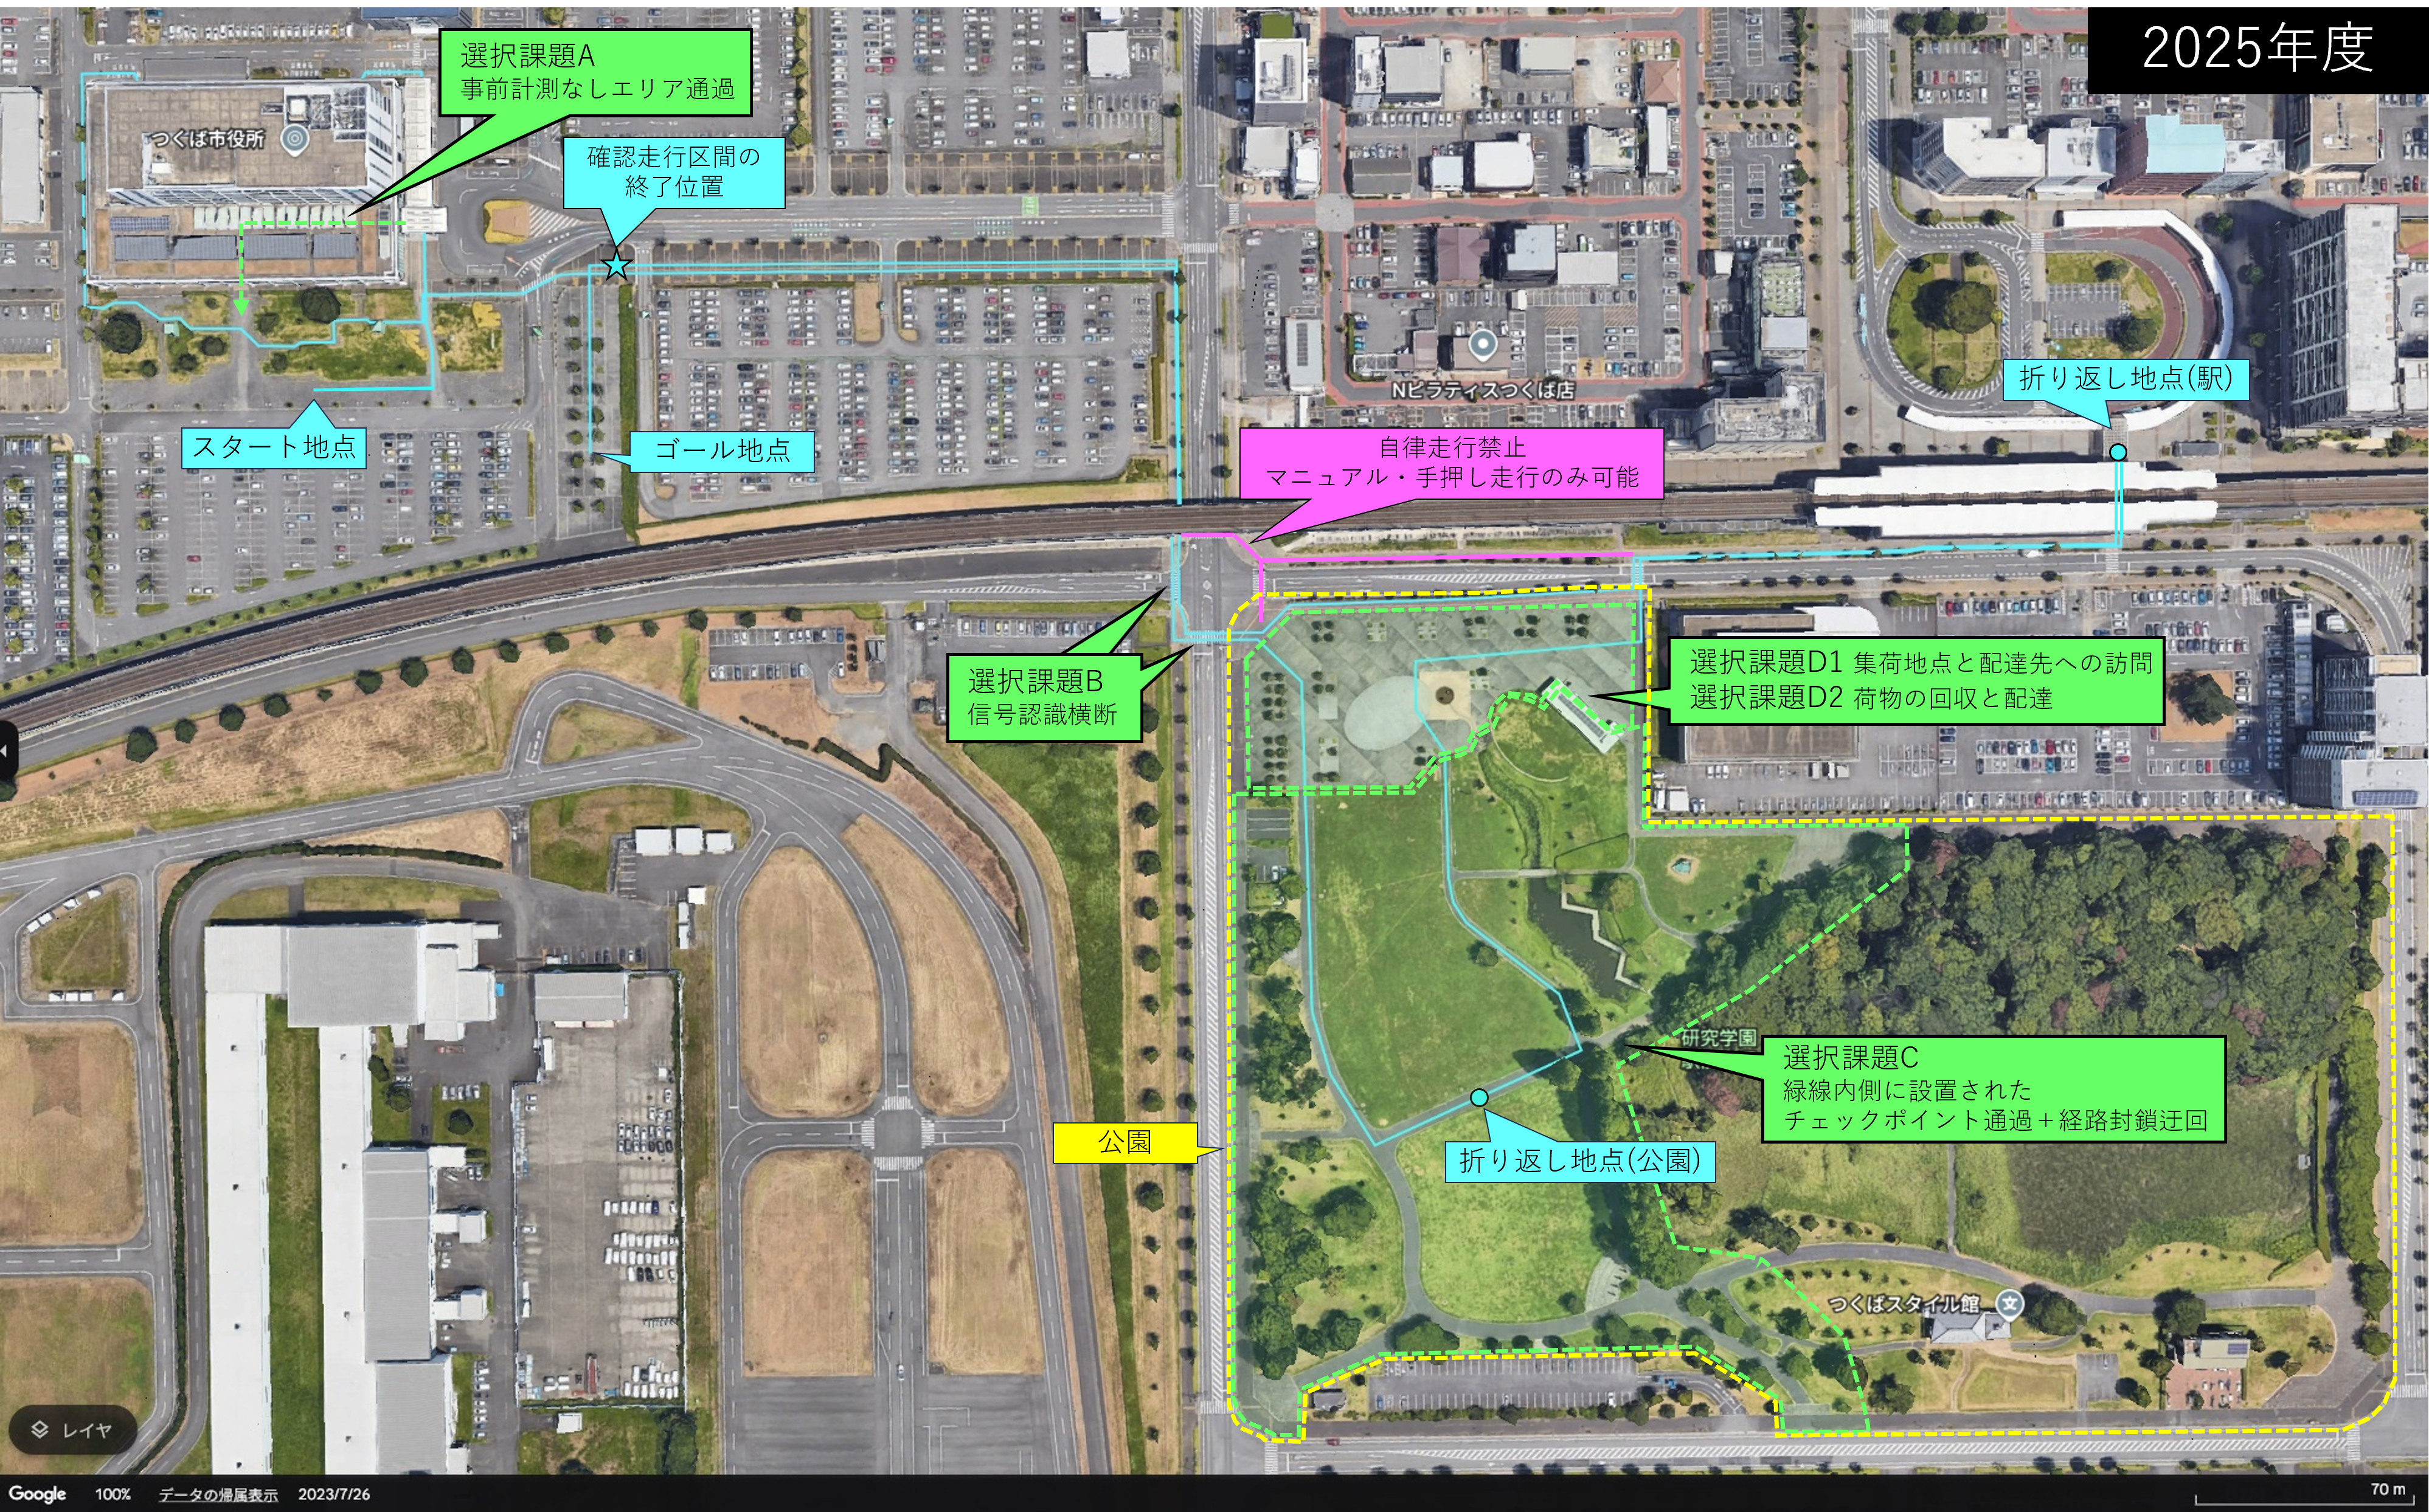
\includegraphics[keepaspectratio, scale=0.3]
      {images/course_2025.png}
 \caption{Course map of the Tsukuba Challenge 2025(souce: \cite{つくばチャレンジ})}
 \label{Fig:Course map of the Tsukuba Challenge 2025}
\end{figure}

\newpage
\section{実験結果}
% 表
\tabref{}に示すように, 
% 6
\chapter{結論}
本研究では, ROSベースの自律移動ロボットのナビゲーションにおけるパラメータ調整手順を整理したドキュメントを作成し, その有効性を検証した. 
ドキュメントはROS Navigation stackのパラメータを中心に構成されている. 
津田沼チャレンジの実験では, 作成者自身および学部3年生のいずれもがそのコースを完走し, ドキュメントの妥当性が確認された. 
また, つくばチャレンジ2025において, 
%
%% Main Matter
\mainmatter{}
%
% 1
\chapter{序論}
\label{chap:introduction}
%
%\input{introduction/preface}
%
%!TEX root = ../thesis.tex

\section{背景}
近年, ROS(Robot Operating System)をベースとした自律移動ロボットのナビゲーション技術が, 警備ロボットや案内ロボットなど, 様々な分野で活用されつつある. 
ただし, ナビゲーションにおいては, ROS Navigation stackのパラメータ, オドメトリ調整のパラメータ, 地図生成のパラメータなど, 複数のパラメータを
適切に調整しなければ自律移動を行うことができない. 

また, 現状ではこれらのパラメータ調整に関する明確な指針は十分に示されていない. 
特に, インターネット上で公開されている情報の多くは屋内環境やシミュレータを対象したものであり, 
センサ誤差や環境変動が大きく調整が困難な屋外環境かつ実ロボットに特化した情報は少ないという課題がある. 
そのため, 屋外環境かつ実ロボットにも対応したナビゲーションにおけるパラメータ調整手順の明確化が求められる. 
\newpage
\section{関連研究}
ROSのナビゲーションのパラメータ調整について解説されている関連研究として, Kaiyu ZhengによるROS Navigation Tuning Guideが挙げられる. 
このガイドは, ROS Navigation stackの性能を最大化するためのパラメータ調整プロセスを解説するものであり, AMCLやMove Baseなど, ナビゲーションにおける主要な項目を網羅している. 

しかし, \figref{Fig:laser-related parameters}, \figref{Fig:odometry and particle filter parameters}のように具体的なパラメータ値が提示され, それらが望ましい設定値であると示している. 
そのため, 自己位置推定のずれや経路計画の失敗など, 特定の環境や問題に直面した際に, どのパラメータをどのように調整すべきかという手順までは明確に示されていない. 
読み手はパラメータに関数する知見は得られるものの, 全体としてナビゲーションシステムを最適化していく具体的な調整フローを導き出すのは難しいという課題がある. 
\begin{figure}[hbtp]
  \centering
 \includegraphics[keepaspectratio, scale=0.3]
      {images/senkou_1.png}
 \caption{laser-related parameters}
 \label{Fig:laser-related parameters}
\end{figure}

\begin{figure}[hbtp]
  \centering
 \includegraphics[keepaspectratio, scale=0.3]
      {images/senkou_2.png}
 \caption{odometry and particle filter parameters}
 \label{Fig:odometry and particle filter parameters}
\end{figure}
%\subsubsection{etc...}
\newpage
\section{目的}
本論文では, ロボットにおけるナビゲーションの調整手順を体系化し, 適切な調整方法を明らかにすることを目的とする. 

\section{論文の構成}
本論文では以下のように構成される. 

2章で本研究で使用される要素技術について述べる. 

3章では本研究で作成したドキュメントについて述べる. 

4章では

5章では

\newpage

% 2
\chapter{要素技術}
\section{ROS}
ROS(Robot Operating System)は, ロボット開発を効率化するためのオープンソースソフトウェアフレームワークである. 
複数のプログラミング言語向けのライブラリや, センサや状態を可視化するツール群, ノード間のメッセージ通信機構, およびパッケージによるモジュール管理機能を備えている点が特徴である. 
ROSにおける基本的な実行単位はノードであり, ノードはトピックやサービスといった仕組みを通じて情報を交換する. 
これにより, センサデータの取得や制御アルゴリズム, 経路計画などを個別のモジュールとして構成し, 分散して動作させることが可能となる. 
さらに, 既成のアルゴリズムやデバイス向けソフトウェアをパッケージとして利用することで, 開発者は低コストかつ短期間で複雑な機能を実装することができる. 

\section{オドメトリ}
オドメトリは, ロボットが自己位置を推定するための基礎的な手法であり, 車輪の回転量から移動距離および姿勢変化を算出する技術である. 
具体的には, エンコーダによって取得される各車輪の回転角度から, ロボットの並進移動量および回転角度を求めることで, 
時系列的にロボットの位置を更新していく. 
この手法は, 外部装置に依存せずに, 連続的な位置推定が可能であるため, 自己位置推定や経路追従制御における基本情報として広く用いられている. 
しかし, 車輪の空転やスリップ, 床面の凹凸などによって誤差が累積するという問題があり, 長時間の走行では位置ずれが大きくなる傾向がある. 
そのため, ロボットの車輪間距離や各車輪径などのパラメータを事前に調整する必要がある. 

\section{ナビゲーション}
ROS Navigation stack\cite{navstack}は, 自律移動ロボットが環境内を自律的に移動するためのソフトウェアフレームワークである. 主に以下の要素から構成されている. 
\begin{itemize}
     \item \textbf{自己位置推定}\\
     ロボットの現在位置を推定する代表的な手法として, AMCL(Adaptive Monte Carlo Localization)が用いられる. 
     AMCLはROS Navigation Stackで自己位置推定を行う確率的アルゴリズムであり, LiDARやオドメトリ情報をもとに多数の仮説(パーティクル)を生成し, 
     それぞれの重みを更新することでロボットの位置を推定する. また, 状況に応じてパーティクル数を動的に調整することで精度と計算負荷のバランスを取る特徴をもつ. 
     一方で, その性能はオドメトリ誤差やレーザノイズなど多くのパラメータ設定に依存しており, 実環境に応じたチューニングが重要となる. 
     \figref{Fig:lamcl_example}に自己位置推定の様子を示す. 
     \begin{figure}[hbtp]
     \centering
          \includegraphics[keepaspectratio, scale=0.2]
           {images/amcl_example.png}
          \caption{Localization in Rviz}
          \label{Fig:lamcl_example}
     \end{figure}

     \item \textbf{地図生成}\\
     未知領域においては, 環境のマッピングのため, SLAM(Simultaneous Localization and Mapping)が必要となる. 
     SLAMは, ロボットが未知の環境内で自己位置を推定しながら同時に地図を生成するための手法であり, 
     自律移動の基盤技術の一つである. ロボットはLiDARやカメラなどのセンサ情報を取得し, 環境内の特徴点や障害物を検出することで地図を構築すると同時に, 
     自身の位置をその地図上で推定する. この相互依存的な推定を繰り返すことで, 外部基準を持たない環境でも自己位置と地図を同時に確立できる. 
     \figref{Fig:Map}にSLAMで作成された地図を示す. 
     \begin{figure}[hbtp]
     \centering
          \includegraphics[keepaspectratio, scale=0.2]
           {images/slam_toolbox.png}
          \caption{Map created with SLAM}
          \label{Fig:Map}
     \end{figure}

     \item \textbf{経路計画}\\
     経路計画は, ロボットが目的地へ到達するための経路を生成, 追従するプロセスであり, ナビゲーションシステムの中心的な役割を担う. 
     大域的経路計画は, 静的な地図情報をもとに, ロボットの現在位置から目的地までの全体的な経路を計算する段階である. 
     ここでは主にDijkstra法やA*アルゴリズムといったグラフ探索手法が用いられ, 障害物を避けつつコストマップ上で最短または最適な経路を算出する. 
     一方, 局所的経路計画は, ロボットが実際に移動する際の動作をリアルタイムに制御する段階であり, 
     センサ情報をもとに動的な障害物を回避しながら経路を追従する. 
     代表的な手法であるDWA(Dynamic Window Approach)は, ロボットの運動学的制約を考慮しつつ, 
     速度空間内で安全かつ効率的な制御コマンドを探索するアルゴリズムである. 
     DWAは目標方向の進行性, 障害物との距離, 安全性など複数の評価関数を組み合わせて最適な行動を選択することで, 
     滑らかな走行と衝突回避を両立させている. 
     \item \textbf{コストマップ}\\
     コストマップは, ロボットの経路計画において基盤となる情報構造であり, 環境内の障害物や走行困難な領域を数値化して表現することで, 
     経路計画アルゴリズムが安全かつ効率的に移動できるようにする. 
     ROS Navigation stackでは, コストマップは, 静的マップと動的マップにに分けて管理される. 
     静的マップはあらかじめ生成された地図に基づく固定的な障害物情報を提供し, 
     局所的な経路計画や障害物回避の基盤として利用される. 
     一方, 動的マップはLiDARやカメラなどのセンサ情報をもとにリアルタイムで更新され, 
     移動中に出現する人などの動的障害物を反映する. コストマップ上では, 
     障害物が存在するセルの値が高く, 通行可能な領域は低い値で表現される. 
     この数値は経路計画アルゴリズムによって考慮され, ロボットはより安全でコストの低い経路を優先して移動する. 
     これにより, 経路計画は単に障害物を避けるだけでなく, 走行中の安全性を確保しつつ目標地点まで到達できるようになる. 
     \figref{Fig:costmap}にコストマップの一例を示す. 
     \begin{figure}[hbtp]
     \centering
          \includegraphics[keepaspectratio, scale=0.2]
           {images/costmap.png}
          \caption{Costmap in Rviz}
          \label{Fig:costmap}
     \end{figure}     
\end{itemize}
% 3
\chapter{ドキュメント}
\section{ドキュメントの構成}
作成したドキュメント(\url{https://github.com/open-rdc/nav_tuning_guide})の構成は以下の要素から構成されている. 
また, 作成にあたってROS WikiのNavigationページを参考にした.
\cite{ros_wiki_navigation}
\begin{itemize}
     \item \textbf{自己位置推定(AMCL)}
     \begin{itemize}
        \item \textbf{必要最小限の設定}
        \item \textbf{主要パラメータの調整}
        \item \textbf{その他パラメータの調整}
        \item \textbf{ROS\_ERRORが出たときの問題と対処法}
    \end{itemize}
     \item \textbf{経路計画(Move Base)}
    \begin{itemize}
        \item \textbf{必要最小限の設定}
        \item \textbf{Move Baseの基本となるパラメータ調整}
        \item \textbf{リカバリ動作のパラメータ調整}
        \item \textbf{コストマップのパラメータ調整}
        \item \textbf{ローカルプランナーのパラメータ調整}
        \item \textbf{グローバルプランナーのパラメータ調整}
        \item \textbf{ROS\_WARNが出たときの問題と対処法}
    \end{itemize}
\newpage
     \item \textbf{地図}
    \begin{itemize}
        \item \textbf{地図作成方法に関して}
        \item \textbf{slam\_toolboxでの地図作成方法}
        \item \textbf{glimでの地図作成方法}
        \item \textbf{大規模屋外環境での地図解像度設定}
    \end{itemize}
    \item \textbf{オドメトリ}
    \begin{itemize}
        \item \textbf{オドメトリの調整手順}
    \end{itemize}     
\end{itemize}

\section{ドキュメントの例}
本論文では, 作成したドキュメントの中から例として, オドメトリ調整と自己位置推定(AMCL), コストマップ, 地図の
4項目を取り上げ, 記載内容の一部を示す. 

\subsection{オドメトリ調整}
調整対象のパラメータは, 車輪半径に関する補正係数であるwheel\_radius\_multiplierと, 車輪環距離に関する補正係数であるwheel\_separation\_multiplierの2つである. 
これらはロボットのオドメトリの正確さに直結するため, 自己位置推定を行う上で最初に調整すべき項目である. 

調整手順は以下の通りである. まず, Rvizを用いてトピックの可視化の準備を行う. 固定座標系をodomに設定し, LaserScanトピックを表示することで, ロボットの移動に伴うセンサ計測をできるようにする. 

次に, ロボットを壁から数メートル離れた位置に配置し, 直進させて並進成分の正確さを確認する. 
このとき, 得られるレーザスキャンに厚みが生じる場合は, wheel\_radius\_multiplierを調整する. 

さらに, ロボットをその場で回転させ, 回転成分の正確さを確認する. 
スキャンが1〜2度以上ずれている場合は, wheel\_separation\_multiplierを調整する. 
最後に再度直進させ, 並進と回転の双方でスキャンが一致していることを確認した時点で調整を完了とする. 

\figref{fig:Scanvisualizedinrviz}にオドメトリ調整前後のレーザスキャンをRvizで可視化した様子を示す. 
\begin{figure}[h]
     \centering
     \begin{minipage}[c]{65mm}
         \centering
         \includegraphics[height=40mm]{images/before_odom.png}
         \subcaption{Before odometry adjustment}
     \end{minipage}
     \begin{minipage}[c]{65mm}
         \centering
         \includegraphics[height=40mm]{images/after_odom.png}
         \subcaption{After odometry adjustment}
     \end{minipage}
     \caption{Scan visualized in Rviz}
     \label{fig:Scanvisualizedinrviz}
\end{figure}

\subsection{AMCLにおけるオドメトリ関連パラメータの調整}
自己位置推定に用いるAMCLにおいて, 最初に調整すべきパラメータはodom\_alpha1〜odom\_alpha4である. 
これらはオドメトリの信頼度を決定する値であり, 大きな値を設定すると, オドメトリに含まれるノイズが大きいとみなされ, オドメトリの影響が小さくなる. 
一方で, 小さな値を設定するとオドメトリを強く信頼するようになる. 屋外環境ではオドメトリ誤差が大きくなるため, パラメータを過度に小さくすると誤推定に繋がる危険がある. 
特にodom\_alpha2とodom\_alpha3の調整が有効である. 

調整方法は以下の通りである. まず, 走行データをrosbagで記録し, Rvizを用いてパーティクルの散らばりや自己位置のずれ方を可視化する. 
これにより, どのパラメータが問題に寄与しているかを予測できる. その後, 記録したデータを再生し, パラメータを変更しながらオフラインでAMCLを動作させることで, パーティクルの挙動を確認できる. 

調整の基準としては, スキャンデータと地図の対応関係を利用する. 例えば, \figref{Fig:tate}に示すように, スキャンが並進方向にずれる場合はodom\_alpha3を増加させることで改善できる. 
また, \figref{Fig:kaiten}のように, 回転方向にずれる場合はodom\_alpha2を増加させることで修正を試みる. 
\figref{Fig:hatan}に示すように, 自己位置が徐々にずれていく場合には, odom\_alpha1〜odom\_alpha4させることで安定化を図る. 
特に, alpha2とalpha3の調整が有効である. 
\begin{figure}[H]
  \centering
 \includegraphics[keepaspectratio, scale=0.13]
      {images/tate.png}
 \caption{Example of translational drift}
 \label{Fig:tate}
\end{figure}
\begin{figure}[H]
  \centering
 \includegraphics[keepaspectratio, scale=0.15]
      {images/kaiten.png}
 \caption{Example of rotational drift}
 \label{Fig:kaiten}
\end{figure}
\begin{figure}[H]
  \centering
 \includegraphics[keepaspectratio, scale=0.15]
      {images/jikoitihatann.png}
 \caption{Example of localization failure}
 \label{Fig:hatan}
\end{figure}

調整完了の基準としては, コントローラ操作時のrosbagを再生した際に自己位置の破綻がなく, かつ実ロボットによる自律走行においてもゴールまで破綻なく移動できることである. 

さらに, AMCLの調整においては, 地図とオドメトリのどちらを信頼するかというトレードオフが存在する. 
地図が高精度で環境と一致している場合には, スキャンマッチングが有効に働くため, odom\_alphaを大きめに設定しても安定した推定が得られる. 
一方で, 地図の精度が低い場合や環境変動が大きい場合には, オドメトリを相対的に信頼する方が安定する. 
ただし, オドメトリへの依存度を上げすぎると, 特に屋外環境では累積誤差によって自己位置が破綻する危険がある. 
このように, 状況に応じてバランスを取ることが, AMCLのパラメータ調整の難しさであるといえる. 

\figref{fig:ScanandMap}にAMCL調整前後のレーザスキャンと地図をRvizで可視化した様子を示す.
\begin{figure}[H]
     \centering
     \begin{minipage}[c]{65mm}
         \centering
         \includegraphics[height=40mm]{images/scanmap_before.png}
         \subcaption{Before AMCL adjustment}
     \end{minipage}
     \begin{minipage}[c]{65mm}
         \centering
         \includegraphics[height=40mm]{images/scanmap_after.png}
         \subcaption{After AMCL adjustment}
     \end{minipage}
     \caption{Map and scan visualized in Rviz}
     \label{fig:ScanandMap}
\end{figure}

\subsection{コストマップのパラメータ調整}
costmapは, ロボットの周囲環境を表現する重要なマップである. デフォルト設定のままでも動作は可能であるが, 
障害物回避性能や応答性を向上させたい場合には, 各種パラメータを調整することが有効である. 

costmapにはlocal\_costmapとglobal\_costmapの2種類が存在し, 両者で共通するパラメータが多い. 
しかし, 名前空間ごとに独立してパラメータを定義することで, それぞれの役割に適した設定値を与えることが可能である. 
また, 名前空間で個別に値を指定しなかった場合には, そのパラメータ値がlocal\_costmapとglobal\_costmapの両方に適用される. 

まず, local\_costmapの主なパラメータについて述べる. update\_frequency は地図の更新頻度を表し, 
値を大きくしすぎると動的障害物の変化を適切に反映できなくなる可能性がある. 
一方で, 小さくしすぎるとCPU負荷が増大し, 処理が滞る可能性がある. 
また, この値が適切でない場合には, 実行時にROSWARNが出るため注意が必要である. 

local\_costmapの幅と高さを設定するwidthとheightは, \figref{Fig:lmap}に示すように, ロボット周辺に生成される局所領域の大きさを規定する. 
値を大きくするほど広範囲の障害物情報を取り込めるが, その分だけ計算量は増加する. 
\begin{figure}[H]
  \centering
 \includegraphics[keepaspectratio, scale=0.15]
      {images/localcostmap.png}
 \caption{Local\_costmap}
 \label{Fig:lmap}
\end{figure}

inflation\_radiusは障害物をどの程度膨張させるかを決定するパラメータである. 
障害物セルから周囲に, コストを膨張させる値であり, 安全な経路を生成する際に重要となる. 
inflation\_radiusに加えて, cost\_scaling\_factorを用いることで, 膨張したコストの減衰具合を調整することができる. 
cost\_scaling\_factorの値を大きくしすぎると, inflation\_radiusを変更しても, 
実際にコストが膨張する範囲が極端に狭くなるため, 注意が必要である. 
\figref{Fig:cost1}, \figref{Fig:cost10}, \figref{Fig:cost20}にinflation\_radiusの値を固定し, 
cost\_scaling\_factorの値を変更したときのコストの膨張具合を示す. 
\begin{figure}[H]
  \centering
 \includegraphics[keepaspectratio, scale=0.13]
      {images/costsca1.png}
 \caption{Inflated obstacles at cost\_scaling\_factor=1}
 \label{Fig:cost1}
\end{figure}
\begin{figure}[H]
  \centering
 \includegraphics[keepaspectratio, scale=0.13]
      {images/costsca10.png}
 \caption{Inflated obstacles at cost\_scaling\_factor=10}
 \label{Fig:cost10}
\end{figure}
\begin{figure}[H]
  \centering
 \includegraphics[keepaspectratio, scale=0.13]
      {images/costsca20.png}
 \caption{Inflated obstacles at cost\_scaling\_factor=20}
 \label{Fig:cost20}
\end{figure}

resolutionはcostmapを構成する1セルおける大きさを示す値であり, 小さくするほど高精細な地図となる一方, 
計算量は増加する. 逆に, resolutionを大きくすると粗い地図となり計算量を削減できるが, 
障害物の形状が不正確になる可能性がある. 
\figref{Fig:re1}, \figref{Fig:re01}, \figref{Fig:re05}に異なるresolutionにおけるコストマップを示す. 
\begin{figure}[H]
  \centering
 \includegraphics[keepaspectratio, scale=0.13]
      {images/re_001.png}
 \caption{Costmap at resolution=0.01}
 \label{Fig:re1}
\end{figure}
\begin{figure}[H]
  \centering
 \includegraphics[keepaspectratio, scale=0.13]
      {images/re_01.png}
 \caption{Costmap at resolution=0.1}
 \label{Fig:re01}
\end{figure}
\begin{figure}[H]
  \centering
 \includegraphics[keepaspectratio, scale=0.13]
      {images/re_05.png}
 \caption{Costmap at resolution=0.5}
 \label{Fig:re05}
\end{figure}

次に, global\_costmapについて述べる. 
上記で述べたパラメータはlocal\_costmapと同様の意味を持つ. 
しかし, inflation\_radiusに関しては, local\_costmapと異なり, 
static\_layerによって読み込まれた静的マップ全体に対して膨張処理が適用される点に特徴がある. 
\figref{Fig:gmap}にglobal\_costmapの一例を示す. 
\begin{figure}[H]
  \centering
 \includegraphics[keepaspectratio, scale=0.13]
      {images/globalcostmap.png}
 \caption{Global\_costmap}
 \label{Fig:gmap}
\end{figure}

以上のように, costmapのパラメータはロボットの経路計画と障害物回避性能に直接影響するため, 
環境に応じた調整が必要となる. 

%\newpage
\subsection{大規模屋外環境での地図解像度設定}
つくばチャレンジ\cite{つくばチャレンジ}のような大規模な屋外環境における自律移動では, 
使用する地図の総セル数が非常に大きくなる. このとき, 経路計画で用いられる Dijkstra 法の計算量は, 
地図の総セル数に強く依存する. そのため, セル数が増大すると計算負荷が高まり, 
ロボットが停止を繰り返すなどの問題が生じることがある. 実際に, 
つくばチャレンジ2025の初回実験走行では, 計算領域が過大であったために, 
ロボットが断続的に停止する様子が確認された. 

ROSのmap\_serverが扱う地図は格子状のセルで構成されており, 1セルが表す物理距離は
解像度(resolution)によって定義される. 解像度を大きく設定すると, 1セルあたりの距離が
広がり, 結果として地図全体のセル数が減少する. 例えば, resolutionを0.10から0.20に変更した
場合, 格子は荒くなるが, 総セル数は大きく減少し, 経路計画の計算速度は向上する. 
\tabref{tab:resolution_comparison}に異なる解像度における特性の比較を示す. 
\begin{table}[H]
  \centering
  \caption{Comparison of characteristics for different map resolutions}
  \label{tab:resolution_comparison}
  \begin{tabular}{lcc}
    \hline
    & \textbf{Low resolution} & \textbf{High resolution} \\
    \hline
    Grid granularity & Fine & Coarse \\
    Number of total cells & Large & Small \\
    Computational cost & High & Low \\
    \hline
  \end{tabular}
\end{table}

つくばチャレンジ2025においては, 地図のスケールを調整した. 
その結果を, \tabref{tab:tsukuba2025_map_scale}に示す. 調整により, 総計算領域を約65\%削減することができた. 
この削減により, Dijkstra 法による経路探索の計算量が大幅に低減し, ロボットが停止を繰り返す問題を解消することができた. 
\figref{Fig:beforemap}, \figref{Fig:aftermap}にスケールを統一した調整前, 調整後の地図を示す. 

ただし, 解像度を過度に大きくすると, 地図が粗くなることで自己位置推定が不安定になる場合や, 
狭い通路がセルの粗さによって潰され, 通行不可能と判断される場合がある. そのため, 
解像度は単に大きくすればよいというものではないことを注意する必要がある. 
\begin{table}[htbp]
  \centering
  \caption{Comparison of map scale adjustment in Tsukuba Challenge 2025}
  \label{tab:tsukuba2025_map_scale}
  \begin{tabular}{lccc}
    \hline
     & Image size [pixel] & Total number of cells & resolution \\
    \hline
    Before adjustment & 7077 $\times$ 3773 & Approx.\ 26.69 million & 0.10 \\
    After adjustment  & 4163 $\times$ 2219 & Approx.\ 9.24 million & 0.17 \\
    \hline
  \end{tabular}
\end{table}

\begin{figure}[hbtp]
  \centering
 \includegraphics[keepaspectratio, scale=0.05]
      {images/tsukuba_all_2_edit_12_edit_14.png}
 \caption{Map before adjustment}
 \label{Fig:beforemap}
\end{figure}
\begin{figure}[hbtp]
  \centering
 \includegraphics[keepaspectratio, scale=0.05]
      {images/tsukuba_all_2_edit_12_edit_14_re_17.png}
 \caption{Map after adjustment}
 \label{Fig:aftermap}
\end{figure}


% 4
\chapter{津田沼チャレンジによるドキュメントの有効性の検証実験}
\section{実験概要}
本研究で作成したドキュメントの有用性を確認するため, 津田沼チャレンジ\cite{tsudachare}のコースを用いて自律移動実験を行った. 
実験では, ドキュメントによる手順通りにナビゲーションのパラメータを調整されたロボットが, 自律的に設定されたコースを完走できるかで, ドキュメントの有用性を確認することを目的とした. 

検証のため以下の2つの実験を行った. 
\begin{table}[H]
     \centering
     \begin{tabular}{ll}
         $実験1$ & ドキュメント作成者が2025年度版コースを対象として行った有用性の検証 \\
         $実験2$ & ROS初心者の学部3年生が2024年度版コースを対象として行った有用性の検証 \\
     \end{tabular}
\end{table}
%実験は, ドキュメント作成者が2025年度版コースで行ったものと, ROS初心者の学部3年生がドキュメントを参照して2024年度版コースで行ったものの2種類である. 
それぞれのコースを\figref{Fig:Course map of the Tsudanuma Challenge 2025}, \figref{Fig:Course map of the Tsudanuma Challenge 2024}に示す.
実験1では, 走行地図の作成から自己位置推定および経路計画に関する各種パラメータの調整までを全て行った. 
また, 2025年8月27日に行われた実験1の本走行においては, LiDARの計測値が一定の閾値以下になったときに減速, 停止を行う処理や, 
特定の場所で一時的にコストマップを無効化する処理, ロボットがスタックしたときにコストマップを初期化する処理といった補助的なノードを併用した. 
これらは, 第5章にて述べる, 人やロボットなどの動的障害物が多いつくばチャレンジ\cite{つくばチャレンジ}を見据えた自律移動上の拡張機能として導入した. 
一方, 実験2では, 作成者がまとめたドキュメントを基に, 作成者が作成した地図を使用してナビゲーションのパラメータ調整を行った. 
また, パラメータ調整に要した時間についても記録し, 調整の負担を把握する参考とした. 

実験には, 本研究室で開発されているロボットORNE-box2\cite{井口颯人2023屋外自律移動ロボットプラットフォーム-orne}を使用した. 
その外観を\figref{Fig:ORNE-box2}に示す. 
また, ナビゲーションにはROS Navigation stackを用いた. ORNE-box2を含めたそのシステム構成を\figref{Fig:system}に示す. 
ORNE-box2はPCとしてJetson AGX Xavier (32GB RAM)を搭載しており, 
3D-LiDAR (R-Fans-16), 2D-LiDAR (UTM-30LX-EW), IMU (ADIS16470), およびエンコーダを備えている. 
2D-LiDARは障害物検出に使用し, 3D-LiDARは自己位置推定に用いた. 
IMUとエンコーダに基づくオドメトリはジャイロオドメトリとして統合し, AMCLに対して移動情報を提供している. 
ナビゲーションシステムは, Map Serverが提供する静的地図を基にAMCLが自己位置を推定し, Move Baseが経路計画を行い, 速度指令値を送信する構成である. 
また, Waypoint Serverは, あらかじめ設定した複数の目的地を管理し, 各地点に到達するごとにMove Baseに対して次の目的地を送信することで, 
指定されたコースでの自律移動を実現している. 
\begin{figure}[hbtp]
  \centering
 \includegraphics[keepaspectratio, scale=0.5]
      {images/2025tsudacha.png}
 \caption{Course map of the Tsudanuma Challenge 2025 (souce: \cite{tsudachare})}
 \label{Fig:Course map of the Tsudanuma Challenge 2025}
\end{figure}
\begin{figure}[hbtp]
  \centering
 \includegraphics[keepaspectratio, scale=0.5]
      {images/2024tsudacha.png}
 \caption{Course map of the Tsudanuma Challenge 2024 (souce: \cite{tsudachare})}
 \label{Fig:Course map of the Tsudanuma Challenge 2024}
\end{figure}
\begin{figure}[hbtp]
  \centering
 \includegraphics[keepaspectratio, scale=0.4]
      {images/box2.png}
 \caption{ORNE-box2}
 \label{Fig:ORNE-box2}
\end{figure}
\begin{figure}[H]
  \centering
 \includegraphics[keepaspectratio, scale=0.11]
      {images/systembox.png}
 \caption{System configuration}
 \label{Fig:system}
\end{figure}




\newpage
\section{実験結果}
\subsection{実験1}
\begin{table}[H]
  \centering
  \caption{Navigation results of the Tsudanuma Challenge 2025}
  \label{tab:tsudanuma_result}
  \begin{tabular}{lcc}
    \hline
    \textbf{Run type} & \textbf{Number of trials} & \textbf{Number of success} \\
    \hline
    Preliminary run & 10 & 10 \\
    Official run        & 1  & 1  \\
    \hline
  \end{tabular}
\end{table}
\tabref{tab:tsudanuma_result}に示すように, 調整後のシステムを用いて事前走行を10回実施した結果, 
すべての試行でゴールまでの完走を確認した. 
走行コースの全長は約1799m, 走行時間はおよそ40分であり, すべての走行で同区間を完走した. 

さらに, 2025年8月27日に行われた津田沼チャレンジの本走行においてもコースを完走し, 自己位置の破綻や経路追従の失敗は見られなかった. 
本走行での実験風景を\figref{Fig:tsudanumaaa}に示す. 
\begin{figure}[hbtp]
  \centering
 \includegraphics[keepaspectratio, scale=0.2]
      {images/tsudanumachalle.png}
 \caption{Experiment scene}
 \label{Fig:tsudanumaaa}
\end{figure}

\subsection{実験2}
\begin{table}[htbp]
  \centering
  \caption{Navigation results of B3 students in the Tsudanuma Challenge 2024}
  \label{tab:b3_results}
  \begin{tabular}{lccc}
    \hline
     & \textbf{No.1} & \textbf{No.2} & \textbf{No.3} \\
    \hline
    Success & Yes & Yes & Yes \\
    Total time to trial [h] & 5.0 & 3.5 & 4.5 \\
    \hline
  \end{tabular}
\end{table}
\tabref{tab:b3_results}に示すように, ドキュメントの手順に沿ってパラメータ調整を行った結果, 3名ともコースの完走を達成することができた. 
走行コースの全長は約1661m, 走行時間はおよそ35分であり, すべての走行で同区間を完走した. 
いずれの実験においても, ロボットは経路から大きく逸脱することなく目標地点まで走行でき, 安定したナビゲーション動作が確認された. 
また, パラメータ調整に要した時間は3.5〜5.0時間であり, いずれの参加者も作業を完遂することができた. 
これにより, ドキュメントの有用性が数例ではあるが確認された. 



% 5
\chapter{つくばチャレンジによるドキュメントの有効性の検証実験}
\section{実験概要}
本研究で作成したドキュメントの有効性を確認するため, つくばチャレンジ2025\cite{つくばチャレンジ}のコースを用いて自律移動実験を行った. 
実験では, ドキュメントによる手順通りにナビゲーションのパラメータを調整されたロボットが, 自律的に設定されたコースを完走できるかで, ドキュメントの有用性を確認することを目的とした. 
そのコースを\figref{Fig:Course map of the Tsukuba Challenge 2025}に示す.
実験では, 作成者が走行地図の作成から自己位置推定および経路計画に関する各種パラメータの調整までを全て行った. 
また, LiDARの計測値が一定の閾値以下になったときに減速, 停止を行う処理や, 
特定の場所で一時的にコストマップを無効化する処理, ロボットがスタックしたときにコストマップを初期化する処理といった補助的なノードを併用した. これらは, 
人やロボットなどの動的障害物が多いつくばチャレンジにおける自律移動上の拡張として導入した. 

実験には, 本研究室で開発されているロボットORNE-box2を使用した. 
また, ナビゲーションにはROS Navigation stackを用いた. 
\begin{figure}[hbtp]
  \centering
 \includegraphics[keepaspectratio, scale=0.3]
      {images/course_2025.png}
 \caption{Course map of the Tsukuba Challenge 2025(souce: \cite{つくばチャレンジ})}
 \label{Fig:Course map of the Tsukuba Challenge 2025}
\end{figure}

\newpage
\section{実験結果}
% 表
\tabref{}に示すように, 
% 6
\chapter{結論}
本研究では, ROSベースの自律移動ロボットのナビゲーションにおけるパラメータ調整手順を整理したドキュメントを作成し, その有効性を検証した. 
ドキュメントはROS Navigation stackのパラメータを中心に構成されている. 
津田沼チャレンジの実験では, 作成者自身および学部3年生のいずれもがそのコースを完走し, ドキュメントの妥当性が確認された. 
また, つくばチャレンジ2025において, 
%ここにディレクトリのパスを追加していく
%
%% Back Matter
\backmatter{}
%
% 1
\chapter{序論}
\label{chap:introduction}
%
%\input{introduction/preface}
%
%!TEX root = ../thesis.tex

\section{背景}
近年, ROS(Robot Operating System)をベースとした自律移動ロボットのナビゲーション技術が, 警備ロボットや案内ロボットなど, 様々な分野で活用されつつある. 
ただし, ナビゲーションにおいては, ROS Navigation stackのパラメータ, オドメトリ調整のパラメータ, 地図生成のパラメータなど, 複数のパラメータを
適切に調整しなければ自律移動を行うことができない. 

また, 現状ではこれらのパラメータ調整に関する明確な指針は十分に示されていない. 
特に, インターネット上で公開されている情報の多くは屋内環境やシミュレータを対象したものであり, 
センサ誤差や環境変動が大きく調整が困難な屋外環境かつ実ロボットに特化した情報は少ないという課題がある. 
そのため, 屋外環境かつ実ロボットにも対応したナビゲーションにおけるパラメータ調整手順の明確化が求められる. 
\newpage
\section{関連研究}
ROSのナビゲーションのパラメータ調整について解説されている関連研究として, Kaiyu ZhengによるROS Navigation Tuning Guideが挙げられる. 
このガイドは, ROS Navigation stackの性能を最大化するためのパラメータ調整プロセスを解説するものであり, AMCLやMove Baseなど, ナビゲーションにおける主要な項目を網羅している. 

しかし, \figref{Fig:laser-related parameters}, \figref{Fig:odometry and particle filter parameters}のように具体的なパラメータ値が提示され, それらが望ましい設定値であると示している. 
そのため, 自己位置推定のずれや経路計画の失敗など, 特定の環境や問題に直面した際に, どのパラメータをどのように調整すべきかという手順までは明確に示されていない. 
読み手はパラメータに関数する知見は得られるものの, 全体としてナビゲーションシステムを最適化していく具体的な調整フローを導き出すのは難しいという課題がある. 
\begin{figure}[hbtp]
  \centering
 \includegraphics[keepaspectratio, scale=0.3]
      {images/senkou_1.png}
 \caption{laser-related parameters}
 \label{Fig:laser-related parameters}
\end{figure}

\begin{figure}[hbtp]
  \centering
 \includegraphics[keepaspectratio, scale=0.3]
      {images/senkou_2.png}
 \caption{odometry and particle filter parameters}
 \label{Fig:odometry and particle filter parameters}
\end{figure}
%\subsubsection{etc...}
\newpage
\section{目的}
本論文では, ロボットにおけるナビゲーションの調整手順を体系化し, 適切な調整方法を明らかにすることを目的とする. 

\section{論文の構成}
本論文では以下のように構成される. 

2章で本研究で使用される要素技術について述べる. 

3章では本研究で作成したドキュメントについて述べる. 

4章では

5章では

\newpage

% 2
\chapter{要素技術}
\section{ROS}
ROS(Robot Operating System)は, ロボット開発を効率化するためのオープンソースソフトウェアフレームワークである. 
複数のプログラミング言語向けのライブラリや, センサや状態を可視化するツール群, ノード間のメッセージ通信機構, およびパッケージによるモジュール管理機能を備えている点が特徴である. 
ROSにおける基本的な実行単位はノードであり, ノードはトピックやサービスといった仕組みを通じて情報を交換する. 
これにより, センサデータの取得や制御アルゴリズム, 経路計画などを個別のモジュールとして構成し, 分散して動作させることが可能となる. 
さらに, 既成のアルゴリズムやデバイス向けソフトウェアをパッケージとして利用することで, 開発者は低コストかつ短期間で複雑な機能を実装することができる. 

\section{オドメトリ}
オドメトリは, ロボットが自己位置を推定するための基礎的な手法であり, 車輪の回転量から移動距離および姿勢変化を算出する技術である. 
具体的には, エンコーダによって取得される各車輪の回転角度から, ロボットの並進移動量および回転角度を求めることで, 
時系列的にロボットの位置を更新していく. 
この手法は, 外部装置に依存せずに, 連続的な位置推定が可能であるため, 自己位置推定や経路追従制御における基本情報として広く用いられている. 
しかし, 車輪の空転やスリップ, 床面の凹凸などによって誤差が累積するという問題があり, 長時間の走行では位置ずれが大きくなる傾向がある. 
そのため, ロボットの車輪間距離や各車輪径などのパラメータを事前に調整する必要がある. 

\section{ナビゲーション}
ROS Navigation stack\cite{navstack}は, 自律移動ロボットが環境内を自律的に移動するためのソフトウェアフレームワークである. 主に以下の要素から構成されている. 
\begin{itemize}
     \item \textbf{自己位置推定}\\
     ロボットの現在位置を推定する代表的な手法として, AMCL(Adaptive Monte Carlo Localization)が用いられる. 
     AMCLはROS Navigation Stackで自己位置推定を行う確率的アルゴリズムであり, LiDARやオドメトリ情報をもとに多数の仮説(パーティクル)を生成し, 
     それぞれの重みを更新することでロボットの位置を推定する. また, 状況に応じてパーティクル数を動的に調整することで精度と計算負荷のバランスを取る特徴をもつ. 
     一方で, その性能はオドメトリ誤差やレーザノイズなど多くのパラメータ設定に依存しており, 実環境に応じたチューニングが重要となる. 
     \figref{Fig:lamcl_example}に自己位置推定の様子を示す. 
     \begin{figure}[hbtp]
     \centering
          \includegraphics[keepaspectratio, scale=0.2]
           {images/amcl_example.png}
          \caption{Localization in Rviz}
          \label{Fig:lamcl_example}
     \end{figure}

     \item \textbf{地図生成}\\
     未知領域においては, 環境のマッピングのため, SLAM(Simultaneous Localization and Mapping)が必要となる. 
     SLAMは, ロボットが未知の環境内で自己位置を推定しながら同時に地図を生成するための手法であり, 
     自律移動の基盤技術の一つである. ロボットはLiDARやカメラなどのセンサ情報を取得し, 環境内の特徴点や障害物を検出することで地図を構築すると同時に, 
     自身の位置をその地図上で推定する. この相互依存的な推定を繰り返すことで, 外部基準を持たない環境でも自己位置と地図を同時に確立できる. 
     \figref{Fig:Map}にSLAMで作成された地図を示す. 
     \begin{figure}[hbtp]
     \centering
          \includegraphics[keepaspectratio, scale=0.2]
           {images/slam_toolbox.png}
          \caption{Map created with SLAM}
          \label{Fig:Map}
     \end{figure}

     \item \textbf{経路計画}\\
     経路計画は, ロボットが目的地へ到達するための経路を生成, 追従するプロセスであり, ナビゲーションシステムの中心的な役割を担う. 
     大域的経路計画は, 静的な地図情報をもとに, ロボットの現在位置から目的地までの全体的な経路を計算する段階である. 
     ここでは主にDijkstra法やA*アルゴリズムといったグラフ探索手法が用いられ, 障害物を避けつつコストマップ上で最短または最適な経路を算出する. 
     一方, 局所的経路計画は, ロボットが実際に移動する際の動作をリアルタイムに制御する段階であり, 
     センサ情報をもとに動的な障害物を回避しながら経路を追従する. 
     代表的な手法であるDWA(Dynamic Window Approach)は, ロボットの運動学的制約を考慮しつつ, 
     速度空間内で安全かつ効率的な制御コマンドを探索するアルゴリズムである. 
     DWAは目標方向の進行性, 障害物との距離, 安全性など複数の評価関数を組み合わせて最適な行動を選択することで, 
     滑らかな走行と衝突回避を両立させている. 
     \item \textbf{コストマップ}\\
     コストマップは, ロボットの経路計画において基盤となる情報構造であり, 環境内の障害物や走行困難な領域を数値化して表現することで, 
     経路計画アルゴリズムが安全かつ効率的に移動できるようにする. 
     ROS Navigation stackでは, コストマップは, 静的マップと動的マップにに分けて管理される. 
     静的マップはあらかじめ生成された地図に基づく固定的な障害物情報を提供し, 
     局所的な経路計画や障害物回避の基盤として利用される. 
     一方, 動的マップはLiDARやカメラなどのセンサ情報をもとにリアルタイムで更新され, 
     移動中に出現する人などの動的障害物を反映する. コストマップ上では, 
     障害物が存在するセルの値が高く, 通行可能な領域は低い値で表現される. 
     この数値は経路計画アルゴリズムによって考慮され, ロボットはより安全でコストの低い経路を優先して移動する. 
     これにより, 経路計画は単に障害物を避けるだけでなく, 走行中の安全性を確保しつつ目標地点まで到達できるようになる. 
     \figref{Fig:costmap}にコストマップの一例を示す. 
     \begin{figure}[hbtp]
     \centering
          \includegraphics[keepaspectratio, scale=0.2]
           {images/costmap.png}
          \caption{Costmap in Rviz}
          \label{Fig:costmap}
     \end{figure}     
\end{itemize}
% 3
\chapter{ドキュメント}
\section{ドキュメントの構成}
作成したドキュメント(\url{https://github.com/open-rdc/nav_tuning_guide})の構成は以下の要素から構成されている. 
また, 作成にあたってROS WikiのNavigationページを参考にした.
\cite{ros_wiki_navigation}
\begin{itemize}
     \item \textbf{自己位置推定(AMCL)}
     \begin{itemize}
        \item \textbf{必要最小限の設定}
        \item \textbf{主要パラメータの調整}
        \item \textbf{その他パラメータの調整}
        \item \textbf{ROS\_ERRORが出たときの問題と対処法}
    \end{itemize}
     \item \textbf{経路計画(Move Base)}
    \begin{itemize}
        \item \textbf{必要最小限の設定}
        \item \textbf{Move Baseの基本となるパラメータ調整}
        \item \textbf{リカバリ動作のパラメータ調整}
        \item \textbf{コストマップのパラメータ調整}
        \item \textbf{ローカルプランナーのパラメータ調整}
        \item \textbf{グローバルプランナーのパラメータ調整}
        \item \textbf{ROS\_WARNが出たときの問題と対処法}
    \end{itemize}
\newpage
     \item \textbf{地図}
    \begin{itemize}
        \item \textbf{地図作成方法に関して}
        \item \textbf{slam\_toolboxでの地図作成方法}
        \item \textbf{glimでの地図作成方法}
        \item \textbf{大規模屋外環境での地図解像度設定}
    \end{itemize}
    \item \textbf{オドメトリ}
    \begin{itemize}
        \item \textbf{オドメトリの調整手順}
    \end{itemize}     
\end{itemize}

\section{ドキュメントの例}
本論文では, 作成したドキュメントの中から例として, オドメトリ調整と自己位置推定(AMCL), コストマップ, 地図の
4項目を取り上げ, 記載内容の一部を示す. 

\subsection{オドメトリ調整}
調整対象のパラメータは, 車輪半径に関する補正係数であるwheel\_radius\_multiplierと, 車輪環距離に関する補正係数であるwheel\_separation\_multiplierの2つである. 
これらはロボットのオドメトリの正確さに直結するため, 自己位置推定を行う上で最初に調整すべき項目である. 

調整手順は以下の通りである. まず, Rvizを用いてトピックの可視化の準備を行う. 固定座標系をodomに設定し, LaserScanトピックを表示することで, ロボットの移動に伴うセンサ計測をできるようにする. 

次に, ロボットを壁から数メートル離れた位置に配置し, 直進させて並進成分の正確さを確認する. 
このとき, 得られるレーザスキャンに厚みが生じる場合は, wheel\_radius\_multiplierを調整する. 

さらに, ロボットをその場で回転させ, 回転成分の正確さを確認する. 
スキャンが1〜2度以上ずれている場合は, wheel\_separation\_multiplierを調整する. 
最後に再度直進させ, 並進と回転の双方でスキャンが一致していることを確認した時点で調整を完了とする. 

\figref{fig:Scanvisualizedinrviz}にオドメトリ調整前後のレーザスキャンをRvizで可視化した様子を示す. 
\begin{figure}[h]
     \centering
     \begin{minipage}[c]{65mm}
         \centering
         \includegraphics[height=40mm]{images/before_odom.png}
         \subcaption{Before odometry adjustment}
     \end{minipage}
     \begin{minipage}[c]{65mm}
         \centering
         \includegraphics[height=40mm]{images/after_odom.png}
         \subcaption{After odometry adjustment}
     \end{minipage}
     \caption{Scan visualized in Rviz}
     \label{fig:Scanvisualizedinrviz}
\end{figure}

\subsection{AMCLにおけるオドメトリ関連パラメータの調整}
自己位置推定に用いるAMCLにおいて, 最初に調整すべきパラメータはodom\_alpha1〜odom\_alpha4である. 
これらはオドメトリの信頼度を決定する値であり, 大きな値を設定すると, オドメトリに含まれるノイズが大きいとみなされ, オドメトリの影響が小さくなる. 
一方で, 小さな値を設定するとオドメトリを強く信頼するようになる. 屋外環境ではオドメトリ誤差が大きくなるため, パラメータを過度に小さくすると誤推定に繋がる危険がある. 
特にodom\_alpha2とodom\_alpha3の調整が有効である. 

調整方法は以下の通りである. まず, 走行データをrosbagで記録し, Rvizを用いてパーティクルの散らばりや自己位置のずれ方を可視化する. 
これにより, どのパラメータが問題に寄与しているかを予測できる. その後, 記録したデータを再生し, パラメータを変更しながらオフラインでAMCLを動作させることで, パーティクルの挙動を確認できる. 

調整の基準としては, スキャンデータと地図の対応関係を利用する. 例えば, \figref{Fig:tate}に示すように, スキャンが並進方向にずれる場合はodom\_alpha3を増加させることで改善できる. 
また, \figref{Fig:kaiten}のように, 回転方向にずれる場合はodom\_alpha2を増加させることで修正を試みる. 
\figref{Fig:hatan}に示すように, 自己位置が徐々にずれていく場合には, odom\_alpha1〜odom\_alpha4させることで安定化を図る. 
特に, alpha2とalpha3の調整が有効である. 
\begin{figure}[H]
  \centering
 \includegraphics[keepaspectratio, scale=0.13]
      {images/tate.png}
 \caption{Example of translational drift}
 \label{Fig:tate}
\end{figure}
\begin{figure}[H]
  \centering
 \includegraphics[keepaspectratio, scale=0.15]
      {images/kaiten.png}
 \caption{Example of rotational drift}
 \label{Fig:kaiten}
\end{figure}
\begin{figure}[H]
  \centering
 \includegraphics[keepaspectratio, scale=0.15]
      {images/jikoitihatann.png}
 \caption{Example of localization failure}
 \label{Fig:hatan}
\end{figure}

調整完了の基準としては, コントローラ操作時のrosbagを再生した際に自己位置の破綻がなく, かつ実ロボットによる自律走行においてもゴールまで破綻なく移動できることである. 

さらに, AMCLの調整においては, 地図とオドメトリのどちらを信頼するかというトレードオフが存在する. 
地図が高精度で環境と一致している場合には, スキャンマッチングが有効に働くため, odom\_alphaを大きめに設定しても安定した推定が得られる. 
一方で, 地図の精度が低い場合や環境変動が大きい場合には, オドメトリを相対的に信頼する方が安定する. 
ただし, オドメトリへの依存度を上げすぎると, 特に屋外環境では累積誤差によって自己位置が破綻する危険がある. 
このように, 状況に応じてバランスを取ることが, AMCLのパラメータ調整の難しさであるといえる. 

\figref{fig:ScanandMap}にAMCL調整前後のレーザスキャンと地図をRvizで可視化した様子を示す.
\begin{figure}[H]
     \centering
     \begin{minipage}[c]{65mm}
         \centering
         \includegraphics[height=40mm]{images/scanmap_before.png}
         \subcaption{Before AMCL adjustment}
     \end{minipage}
     \begin{minipage}[c]{65mm}
         \centering
         \includegraphics[height=40mm]{images/scanmap_after.png}
         \subcaption{After AMCL adjustment}
     \end{minipage}
     \caption{Map and scan visualized in Rviz}
     \label{fig:ScanandMap}
\end{figure}

\subsection{コストマップのパラメータ調整}
costmapは, ロボットの周囲環境を表現する重要なマップである. デフォルト設定のままでも動作は可能であるが, 
障害物回避性能や応答性を向上させたい場合には, 各種パラメータを調整することが有効である. 

costmapにはlocal\_costmapとglobal\_costmapの2種類が存在し, 両者で共通するパラメータが多い. 
しかし, 名前空間ごとに独立してパラメータを定義することで, それぞれの役割に適した設定値を与えることが可能である. 
また, 名前空間で個別に値を指定しなかった場合には, そのパラメータ値がlocal\_costmapとglobal\_costmapの両方に適用される. 

まず, local\_costmapの主なパラメータについて述べる. update\_frequency は地図の更新頻度を表し, 
値を大きくしすぎると動的障害物の変化を適切に反映できなくなる可能性がある. 
一方で, 小さくしすぎるとCPU負荷が増大し, 処理が滞る可能性がある. 
また, この値が適切でない場合には, 実行時にROSWARNが出るため注意が必要である. 

local\_costmapの幅と高さを設定するwidthとheightは, \figref{Fig:lmap}に示すように, ロボット周辺に生成される局所領域の大きさを規定する. 
値を大きくするほど広範囲の障害物情報を取り込めるが, その分だけ計算量は増加する. 
\begin{figure}[H]
  \centering
 \includegraphics[keepaspectratio, scale=0.15]
      {images/localcostmap.png}
 \caption{Local\_costmap}
 \label{Fig:lmap}
\end{figure}

inflation\_radiusは障害物をどの程度膨張させるかを決定するパラメータである. 
障害物セルから周囲に, コストを膨張させる値であり, 安全な経路を生成する際に重要となる. 
inflation\_radiusに加えて, cost\_scaling\_factorを用いることで, 膨張したコストの減衰具合を調整することができる. 
cost\_scaling\_factorの値を大きくしすぎると, inflation\_radiusを変更しても, 
実際にコストが膨張する範囲が極端に狭くなるため, 注意が必要である. 
\figref{Fig:cost1}, \figref{Fig:cost10}, \figref{Fig:cost20}にinflation\_radiusの値を固定し, 
cost\_scaling\_factorの値を変更したときのコストの膨張具合を示す. 
\begin{figure}[H]
  \centering
 \includegraphics[keepaspectratio, scale=0.13]
      {images/costsca1.png}
 \caption{Inflated obstacles at cost\_scaling\_factor=1}
 \label{Fig:cost1}
\end{figure}
\begin{figure}[H]
  \centering
 \includegraphics[keepaspectratio, scale=0.13]
      {images/costsca10.png}
 \caption{Inflated obstacles at cost\_scaling\_factor=10}
 \label{Fig:cost10}
\end{figure}
\begin{figure}[H]
  \centering
 \includegraphics[keepaspectratio, scale=0.13]
      {images/costsca20.png}
 \caption{Inflated obstacles at cost\_scaling\_factor=20}
 \label{Fig:cost20}
\end{figure}

resolutionはcostmapを構成する1セルおける大きさを示す値であり, 小さくするほど高精細な地図となる一方, 
計算量は増加する. 逆に, resolutionを大きくすると粗い地図となり計算量を削減できるが, 
障害物の形状が不正確になる可能性がある. 
\figref{Fig:re1}, \figref{Fig:re01}, \figref{Fig:re05}に異なるresolutionにおけるコストマップを示す. 
\begin{figure}[H]
  \centering
 \includegraphics[keepaspectratio, scale=0.13]
      {images/re_001.png}
 \caption{Costmap at resolution=0.01}
 \label{Fig:re1}
\end{figure}
\begin{figure}[H]
  \centering
 \includegraphics[keepaspectratio, scale=0.13]
      {images/re_01.png}
 \caption{Costmap at resolution=0.1}
 \label{Fig:re01}
\end{figure}
\begin{figure}[H]
  \centering
 \includegraphics[keepaspectratio, scale=0.13]
      {images/re_05.png}
 \caption{Costmap at resolution=0.5}
 \label{Fig:re05}
\end{figure}

次に, global\_costmapについて述べる. 
上記で述べたパラメータはlocal\_costmapと同様の意味を持つ. 
しかし, inflation\_radiusに関しては, local\_costmapと異なり, 
static\_layerによって読み込まれた静的マップ全体に対して膨張処理が適用される点に特徴がある. 
\figref{Fig:gmap}にglobal\_costmapの一例を示す. 
\begin{figure}[H]
  \centering
 \includegraphics[keepaspectratio, scale=0.13]
      {images/globalcostmap.png}
 \caption{Global\_costmap}
 \label{Fig:gmap}
\end{figure}

以上のように, costmapのパラメータはロボットの経路計画と障害物回避性能に直接影響するため, 
環境に応じた調整が必要となる. 

%\newpage
\subsection{大規模屋外環境での地図解像度設定}
つくばチャレンジ\cite{つくばチャレンジ}のような大規模な屋外環境における自律移動では, 
使用する地図の総セル数が非常に大きくなる. このとき, 経路計画で用いられる Dijkstra 法の計算量は, 
地図の総セル数に強く依存する. そのため, セル数が増大すると計算負荷が高まり, 
ロボットが停止を繰り返すなどの問題が生じることがある. 実際に, 
つくばチャレンジ2025の初回実験走行では, 計算領域が過大であったために, 
ロボットが断続的に停止する様子が確認された. 

ROSのmap\_serverが扱う地図は格子状のセルで構成されており, 1セルが表す物理距離は
解像度(resolution)によって定義される. 解像度を大きく設定すると, 1セルあたりの距離が
広がり, 結果として地図全体のセル数が減少する. 例えば, resolutionを0.10から0.20に変更した
場合, 格子は荒くなるが, 総セル数は大きく減少し, 経路計画の計算速度は向上する. 
\tabref{tab:resolution_comparison}に異なる解像度における特性の比較を示す. 
\begin{table}[H]
  \centering
  \caption{Comparison of characteristics for different map resolutions}
  \label{tab:resolution_comparison}
  \begin{tabular}{lcc}
    \hline
    & \textbf{Low resolution} & \textbf{High resolution} \\
    \hline
    Grid granularity & Fine & Coarse \\
    Number of total cells & Large & Small \\
    Computational cost & High & Low \\
    \hline
  \end{tabular}
\end{table}

つくばチャレンジ2025においては, 地図のスケールを調整した. 
その結果を, \tabref{tab:tsukuba2025_map_scale}に示す. 調整により, 総計算領域を約65\%削減することができた. 
この削減により, Dijkstra 法による経路探索の計算量が大幅に低減し, ロボットが停止を繰り返す問題を解消することができた. 
\figref{Fig:beforemap}, \figref{Fig:aftermap}にスケールを統一した調整前, 調整後の地図を示す. 

ただし, 解像度を過度に大きくすると, 地図が粗くなることで自己位置推定が不安定になる場合や, 
狭い通路がセルの粗さによって潰され, 通行不可能と判断される場合がある. そのため, 
解像度は単に大きくすればよいというものではないことを注意する必要がある. 
\begin{table}[htbp]
  \centering
  \caption{Comparison of map scale adjustment in Tsukuba Challenge 2025}
  \label{tab:tsukuba2025_map_scale}
  \begin{tabular}{lccc}
    \hline
     & Image size [pixel] & Total number of cells & resolution \\
    \hline
    Before adjustment & 7077 $\times$ 3773 & Approx.\ 26.69 million & 0.10 \\
    After adjustment  & 4163 $\times$ 2219 & Approx.\ 9.24 million & 0.17 \\
    \hline
  \end{tabular}
\end{table}

\begin{figure}[hbtp]
  \centering
 \includegraphics[keepaspectratio, scale=0.05]
      {images/tsukuba_all_2_edit_12_edit_14.png}
 \caption{Map before adjustment}
 \label{Fig:beforemap}
\end{figure}
\begin{figure}[hbtp]
  \centering
 \includegraphics[keepaspectratio, scale=0.05]
      {images/tsukuba_all_2_edit_12_edit_14_re_17.png}
 \caption{Map after adjustment}
 \label{Fig:aftermap}
\end{figure}


% 4
\chapter{津田沼チャレンジによるドキュメントの有効性の検証実験}
\section{実験概要}
本研究で作成したドキュメントの有用性を確認するため, 津田沼チャレンジ\cite{tsudachare}のコースを用いて自律移動実験を行った. 
実験では, ドキュメントによる手順通りにナビゲーションのパラメータを調整されたロボットが, 自律的に設定されたコースを完走できるかで, ドキュメントの有用性を確認することを目的とした. 

検証のため以下の2つの実験を行った. 
\begin{table}[H]
     \centering
     \begin{tabular}{ll}
         $実験1$ & ドキュメント作成者が2025年度版コースを対象として行った有用性の検証 \\
         $実験2$ & ROS初心者の学部3年生が2024年度版コースを対象として行った有用性の検証 \\
     \end{tabular}
\end{table}
%実験は, ドキュメント作成者が2025年度版コースで行ったものと, ROS初心者の学部3年生がドキュメントを参照して2024年度版コースで行ったものの2種類である. 
それぞれのコースを\figref{Fig:Course map of the Tsudanuma Challenge 2025}, \figref{Fig:Course map of the Tsudanuma Challenge 2024}に示す.
実験1では, 走行地図の作成から自己位置推定および経路計画に関する各種パラメータの調整までを全て行った. 
また, 2025年8月27日に行われた実験1の本走行においては, LiDARの計測値が一定の閾値以下になったときに減速, 停止を行う処理や, 
特定の場所で一時的にコストマップを無効化する処理, ロボットがスタックしたときにコストマップを初期化する処理といった補助的なノードを併用した. 
これらは, 第5章にて述べる, 人やロボットなどの動的障害物が多いつくばチャレンジ\cite{つくばチャレンジ}を見据えた自律移動上の拡張機能として導入した. 
一方, 実験2では, 作成者がまとめたドキュメントを基に, 作成者が作成した地図を使用してナビゲーションのパラメータ調整を行った. 
また, パラメータ調整に要した時間についても記録し, 調整の負担を把握する参考とした. 

実験には, 本研究室で開発されているロボットORNE-box2\cite{井口颯人2023屋外自律移動ロボットプラットフォーム-orne}を使用した. 
その外観を\figref{Fig:ORNE-box2}に示す. 
また, ナビゲーションにはROS Navigation stackを用いた. ORNE-box2を含めたそのシステム構成を\figref{Fig:system}に示す. 
ORNE-box2はPCとしてJetson AGX Xavier (32GB RAM)を搭載しており, 
3D-LiDAR (R-Fans-16), 2D-LiDAR (UTM-30LX-EW), IMU (ADIS16470), およびエンコーダを備えている. 
2D-LiDARは障害物検出に使用し, 3D-LiDARは自己位置推定に用いた. 
IMUとエンコーダに基づくオドメトリはジャイロオドメトリとして統合し, AMCLに対して移動情報を提供している. 
ナビゲーションシステムは, Map Serverが提供する静的地図を基にAMCLが自己位置を推定し, Move Baseが経路計画を行い, 速度指令値を送信する構成である. 
また, Waypoint Serverは, あらかじめ設定した複数の目的地を管理し, 各地点に到達するごとにMove Baseに対して次の目的地を送信することで, 
指定されたコースでの自律移動を実現している. 
\begin{figure}[hbtp]
  \centering
 \includegraphics[keepaspectratio, scale=0.5]
      {images/2025tsudacha.png}
 \caption{Course map of the Tsudanuma Challenge 2025 (souce: \cite{tsudachare})}
 \label{Fig:Course map of the Tsudanuma Challenge 2025}
\end{figure}
\begin{figure}[hbtp]
  \centering
 \includegraphics[keepaspectratio, scale=0.5]
      {images/2024tsudacha.png}
 \caption{Course map of the Tsudanuma Challenge 2024 (souce: \cite{tsudachare})}
 \label{Fig:Course map of the Tsudanuma Challenge 2024}
\end{figure}
\begin{figure}[hbtp]
  \centering
 \includegraphics[keepaspectratio, scale=0.4]
      {images/box2.png}
 \caption{ORNE-box2}
 \label{Fig:ORNE-box2}
\end{figure}
\begin{figure}[H]
  \centering
 \includegraphics[keepaspectratio, scale=0.11]
      {images/systembox.png}
 \caption{System configuration}
 \label{Fig:system}
\end{figure}




\newpage
\section{実験結果}
\subsection{実験1}
\begin{table}[H]
  \centering
  \caption{Navigation results of the Tsudanuma Challenge 2025}
  \label{tab:tsudanuma_result}
  \begin{tabular}{lcc}
    \hline
    \textbf{Run type} & \textbf{Number of trials} & \textbf{Number of success} \\
    \hline
    Preliminary run & 10 & 10 \\
    Official run        & 1  & 1  \\
    \hline
  \end{tabular}
\end{table}
\tabref{tab:tsudanuma_result}に示すように, 調整後のシステムを用いて事前走行を10回実施した結果, 
すべての試行でゴールまでの完走を確認した. 
走行コースの全長は約1799m, 走行時間はおよそ40分であり, すべての走行で同区間を完走した. 

さらに, 2025年8月27日に行われた津田沼チャレンジの本走行においてもコースを完走し, 自己位置の破綻や経路追従の失敗は見られなかった. 
本走行での実験風景を\figref{Fig:tsudanumaaa}に示す. 
\begin{figure}[hbtp]
  \centering
 \includegraphics[keepaspectratio, scale=0.2]
      {images/tsudanumachalle.png}
 \caption{Experiment scene}
 \label{Fig:tsudanumaaa}
\end{figure}

\subsection{実験2}
\begin{table}[htbp]
  \centering
  \caption{Navigation results of B3 students in the Tsudanuma Challenge 2024}
  \label{tab:b3_results}
  \begin{tabular}{lccc}
    \hline
     & \textbf{No.1} & \textbf{No.2} & \textbf{No.3} \\
    \hline
    Success & Yes & Yes & Yes \\
    Total time to trial [h] & 5.0 & 3.5 & 4.5 \\
    \hline
  \end{tabular}
\end{table}
\tabref{tab:b3_results}に示すように, ドキュメントの手順に沿ってパラメータ調整を行った結果, 3名ともコースの完走を達成することができた. 
走行コースの全長は約1661m, 走行時間はおよそ35分であり, すべての走行で同区間を完走した. 
いずれの実験においても, ロボットは経路から大きく逸脱することなく目標地点まで走行でき, 安定したナビゲーション動作が確認された. 
また, パラメータ調整に要した時間は3.5〜5.0時間であり, いずれの参加者も作業を完遂することができた. 
これにより, ドキュメントの有用性が数例ではあるが確認された. 



% 5
\chapter{つくばチャレンジによるドキュメントの有効性の検証実験}
\section{実験概要}
本研究で作成したドキュメントの有効性を確認するため, つくばチャレンジ2025\cite{つくばチャレンジ}のコースを用いて自律移動実験を行った. 
実験では, ドキュメントによる手順通りにナビゲーションのパラメータを調整されたロボットが, 自律的に設定されたコースを完走できるかで, ドキュメントの有用性を確認することを目的とした. 
そのコースを\figref{Fig:Course map of the Tsukuba Challenge 2025}に示す.
実験では, 作成者が走行地図の作成から自己位置推定および経路計画に関する各種パラメータの調整までを全て行った. 
また, LiDARの計測値が一定の閾値以下になったときに減速, 停止を行う処理や, 
特定の場所で一時的にコストマップを無効化する処理, ロボットがスタックしたときにコストマップを初期化する処理といった補助的なノードを併用した. これらは, 
人やロボットなどの動的障害物が多いつくばチャレンジにおける自律移動上の拡張として導入した. 

実験には, 本研究室で開発されているロボットORNE-box2を使用した. 
また, ナビゲーションにはROS Navigation stackを用いた. 
\begin{figure}[hbtp]
  \centering
 \includegraphics[keepaspectratio, scale=0.3]
      {images/course_2025.png}
 \caption{Course map of the Tsukuba Challenge 2025(souce: \cite{つくばチャレンジ})}
 \label{Fig:Course map of the Tsukuba Challenge 2025}
\end{figure}

\newpage
\section{実験結果}
% 表
\tabref{}に示すように, 
% 6
\chapter{結論}
本研究では, ROSベースの自律移動ロボットのナビゲーションにおけるパラメータ調整手順を整理したドキュメントを作成し, その有効性を検証した. 
ドキュメントはROS Navigation stackのパラメータを中心に構成されている. 
津田沼チャレンジの実験では, 作成者自身および学部3年生のいずれもがそのコースを完走し, ドキュメントの妥当性が確認された. 
また, つくばチャレンジ2025において, 
%

\end{document}
